%% FELthesis: LaTeX class for bachelor, master, and phd thesis in CTU FEL
%% template.tex: template file
%% (c) 2012-2014 Vít Zýka, vit.zyka@seznam.cz
%%
%% 2012-12-17 v0.1 first version derived from cmpthesis.tex

\documentclass[msc, czech]{felthesis} % or [...,czech] for thesis in Czech

%% --- your additional packages:
\usepackage[utf8]{inputenc}

%% --- usefull draft packages
%%\usepackage[notref]{showkeys} % show labels for referencies
%%\usepackage{showlabels}       % similar
%%\usepackage{showidx}          % show index entries on every page
\usepackage{indentfirst}        % odsazeni prvniho odstavce

%% ======================================================== thesis info
\startThesisInfo
  \Title{Metody automatizace testů síťových prvků}
  \Author{Bc. David Felgr}
  \AuthorEmail{felgrdav@fel.cvut.cz} % optional
  \Date{Květen 2015}
  \Department{Katedra Řídící techniky}
  \Advisor{Ing. Pavel Kopecký, doc. Ing. Jiří Novák, Ph.D.}
  \KeywordsCz{Systémové testování, testování založené na modelech, embedded zařízení, automatizované testování.}
  \KeywordsEn{System testing, model based testing, embedded device, automated testing.}
  \AssignmentPage{assignment.pdf} % insert official assignment if given
\stopThesisInfo

%% ============================== your definitions (abbreviations etc.)
%%\def\Ax{\mathbf{A}_{x}}

%% =========================================================== settings
\addbibresource{felgr_david.bib} % bibliography file
\graphicspath{{logo/}{images/}} % subdirectories where TeX finds pictures
\DeclareGraphicsExtensions{.pdf,.png,.jpg}
%% ========================================================== text body
\begin{document}

\MakeTitle

\startFrontMatter
  \startAcknowledgement
Chtěl bych poděkovat svému vedoucímu diplomové práce doc. Ing. Jiřímu Novákovi, Ph.D. za prvotní nasměrování při řešení problému. Dále bych chtěl poděkovat kolegům ve~vývojovém oddělení za cenné rady při realizaci testovacího systému i při jazykové korekci práce.
\stopAcknowledgement

\endinput
%%
%% End of file `acknowledgement.tex'.

  \startDeclaration
\ifCzech
  Prohlašuji, že jsem předloženou práci vypracoval samostatně,
  a~že jsem uvedl veškeré použité informační zdroje v~souladu
  s~Metodickým pokynem o~dodržování etických principů při přípravě
  vysokoškolských závěrečných prací.
\fi
\ifEnglish
  I declare that I worked out the presented thesis independently
  and I quoted all used sources of information in accord with
  Methodical instructions about ethical principles for writing
  academic thesis.
\fi
\stopDeclaration

\endinput
%%
%% End of file `declaration.tex'.

  \startAbstractCz
Tento dokument ukazuje a testuje použití oficiálně doporučené \LaTeX{}ové šablony
\FelThesis{} pro sazbu bakalářské, diplomové a disertační práce na
Elektrotechnické fakultě ČVUT. Šablona definuje všechny povinné
strukturní elementy zmíněných závěrečných prací a formátuje jejich
obsah tak, aby splňovala na škole daná formální pravidla.
\stopAbstractCz

\startAbstractEn
This document shows and tests an usage of the \LaTeX{} officially
recommended design style \FelThesis{} for bachelor (Bsc.), master
(Ing.), or doctoral (Ph.D.) thesis at the Faculty of Electrical
Engineering of the Czech Technical University in Prague.
The template defines all thesis mandatory structural elements and
typesets their content to fulfil the university formal rules.
\stopAbstractEn

\endinput

  \TableOfContents
  \font\mflogo=logo10
\def\METAFONT{{\mflogo META}\-{\mflogo FONT}}
\def\METAPOST{{\mflogo META}\-{\mflogo POST}}
\hyphenation{Post-Script}

\startAbbreviations{%
  As an example of an abbreviation description serve some terms from
  TeX{} world. This introductory paragraph is optional and can stay empty.}
\label{abbrv}%
\abbrv[\TeX{}]  Typesetting program and macro language by Donald Knuth.
\abbrv[\METAFONT{}] Program and macro language for font creation by
  Donald Knuth.
\abbrv[\METAPOST{}] Vector drawing program based on \METAFONT{} with
  Encapsulated PostScript output by John Hobby.
\abbrv[plain \TeX{}]  Original \TeX{} format (macro extension) by
Donald Knuth. User customization is done by programing in \TeX{} macro language.
\abbrv[\LaTeX{}]  Most known and used \TeX{} format originally by
  Leslie Lamport. There is a huge number of packages that extends
  standard functionality or bypass programing in \TeX{}. User
  customization is primarily done by loading predefined class or
  package and rewriting their definitions.
\abbrv[Con\TeX{}t]  Complex typesetting and vector drawing system based
  on \TeX{}, \METAPOST{} and Lua script language by Hans Hagen. Customization is
  done by key-value parametrization with conjunction to \TeX{},
  \METAPOST{} and Lua programing.
\stopAbbreviations

\setlength{\AbbrvIndent}{2em}

\startAbbreviations*[Symbols]{%
  The abbreviation environment starts a new page. If we want to avoid
  page break like in this second short list use starred version {\tt\Backslash
  startAbbreviations*}. Indentation might be adjusted by the command
  {\tt\Backslash setlength\{\Backslash AbbrvIndent\}\{5em\}} to be
  appropriate to the symbols width.}
\abbrv[$\pi$] Final version number of \TeX{}.
\abbrv[e] Final version number of \METAFONT{}.
\abbrv[$2\varepsilon$] Version of today's \LaTeX{} valid since 1994. It
  was intended as a temporary intermediate version between original
  Leslie Lamports's last version \LaTeX{} 2.09 and \LaTeX{}3 that is
  developed as its successor.
\stopAbbreviations

\endinput
%%
%% End of file `abbreviation.tex'.

\stopFrontMatter

\startBodyMatter
  \chapter{Úvod}
Tématem této diplomové práce jsou metody automatizace testů síťových prvků. Nejdříve bychom měl popsat definici testování a různé způsoby jak je možné testování provádět. Definice testování je podle IEEE Software Engineering Body of Knowledge (SWEBOK 2004) následující:

"Softwarové testování se skládá z dynamického ověřování chování programu proti očekávanému chování programu na konečné množině testovacích případů vhodně vybraných z obvykle nekonečné množiny případů."

Na způsoby testování lze pohlížet několika pohledy. Prvním pohledem na testování je rozdělení na šest jednotlivých úrovní testování. Mezi tyto úrovně testování patří testování programátorem, testování jednotlivých jednotek kódu, funkční testování, integrační testování, systémové testování a akceptační testy. Všechny úrovně budou detailně popsány v kapitole používané metody testování. Dalším pohledem na kategorizaci testování je způsob provádění testů. Prvním způsobem je manuální testování, kdy tester manuálně provádí testy podle předem daných testovacích procedur. Dokonalejším způsobem testování je takzvané automatizované testování, kdy testy jsou prováděny automaticky dle předem napsaných testovacích procedur. Testovací procedury jsou psány testery či vývojáři. Všechny testovací procedury musí být přepisovány při změně funkcionality výrobku, nebo při přidání nového výrobku. Tímto přístupem je ušetřeno spoustu času, který byl plýtván opakovaným manuálním testováním identických věcí. Posledním známým a v dnešní době moderním způsobem testování je testování založené na modelech. U tohoto způsobu testování je vytvořen model testované oblasti, či zařízení a automaticky se generují testovací procedury. Způsob testování založeného na modelech ušetří další čas trávený úpravami a tvorbou dalších testovacích procedur při změně funkcionality softwaru či přidání nového produktu, jelikož je upravován pouze model zařízení. Testovací systém, který bude výstupem této diplomové práce, by měl testovat zařízení na úrovni systémového testování. Systémové testy by měl testovací systém pro konkrétní zařízení vybírat a  provádět automatizovaně pomocí testování založeného na modelech.

\section{Praktické využití}
Praktická implementace testovacího systému bude provedena pro testování výrobků společnosti Conel, ze které přišel požadavek na toto zadání. Zadání diplomové práce jsem si vybral, jelikož ve společností pracuji na různých pozicích již 4 roky. Způsoby testování výrobku se během fungování firmy měnily následujícím způsobem. Zpočátku, kdy počet modelů routerů byl velmi malý a routery vyvíjel pouze jeden programátor bylo prováděno pouze testování programátorem a následovali až akceptační testy u zákazníka. Při rostoucím počtu modelů, funkcionalit a počtu vývojářů byl tento systém již dále neudržitelný a mezi testy programátorem a akceptačními testy musely být vloženy systémové testy prováděny testerem podle testovacích procedur. Dnes, kdy počet modelů routerů přesahuje 30 základních modelů a nové funkcionality  přibývají čím dál tím rychleji, je tento systém taktéž dále neudržitelný. Již nyní by kompletní testování všech funkcionalit na všech typech routerů trvalo přibližně měsíc práce v jednom člověku.

\begin{figure}[h]
	\centering
	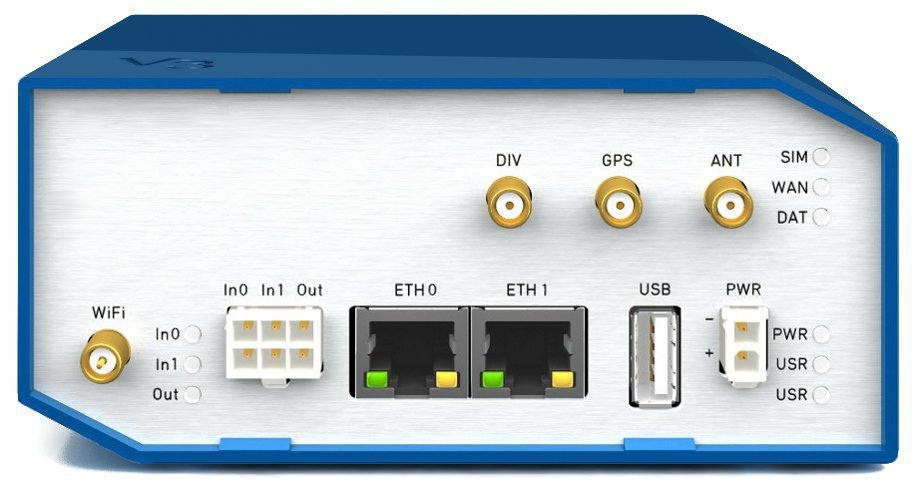
\includegraphics[width=.6\LW]{router}
	\caption{Příklad routeru}
	\label{fig:router}
\end{figure}

Na základě těchto skutečností byl vznešen požadavek na testovací systém, pomocí kterého bude možné automaticky testovat aktuálně vyvíjený firmware na všech vyráběných modelech routerů a jejich volitelných portech. Zvolena byla kombinace integračního testování a testování založené na modelech. Testování bude pokrývat pouze integrační a systémové testování, jelikož z větší části je firmware testovaných výrobků tvořen opensource programy. Psaní unit testů pro každý open source program je časově a složitostně nepřínosné. Systémové testování by mělo probíhat alespoň jednou denně, aby bylo možno případné chyby odchytnout již během vývoje firmwaru a tím usnadnilo a zrychlilo vývoj samotný. Dalším velikým přínosem je zkvalitnění samotného testování, jelikož testovací technici mohou vymýšlet nové testovací procedury a situace, namísto opakovaného manuálního testování stejných procedur.

\section{Aktuálnost}
Testování každého výrobku před uvedením na trh, či testováním nového firmwaru před jeho vydáním je velmi důležitá součást vývoje a neměla by se opomíjet. Hlavním důvodem průběžného testování kompletní funkcionality zařízení je dobré jméno u zákazníka, který nemá zájem o výrobek plný chyb. Dalším důvodem průběžného testování je méně práce pří pozdějším opravování způsobených chyb. Při zvyšování počtu výrobků a funkcionalit je nutné zvyšovat počet testovacích pracovníků, nebo změnit přístup k způsobu testování. Jelikož první řešení se zdá být na první pohled neefektivní, tak se v této práci vydám druhou cestou. Při zvyšování efektivity testů použiju automatizované testování. Dále pokud to bude možné a alespoň trochu efektivní využiji dnes velmi moderní metodu testování založeného na modelech. Každému zařízení by měl být vytvořen model, pomocí kterého budou na určených zařízeních spouštěny vybrané testy s danými parametry. V dnešní době byrokracie tento systém také pomůže ke shromažďování všech testovacích procedur a reportů ze všech provedených testů na jednom místě.

\section{Výstup práce}
Hlavním cílem práce je hotové řešení automatizovaného systémového řešení testování všech modelů bezdrátových routerů společnosti Conel. Výstupem  řešení bude testovací laboratoř obsahující všechny výrobky, pomocné síťové prvky a testovací server. Dalším výstupem bude aplikace na obstarávající režii a spouštění testů, interface pro zobrazování reportů ze všech testů s možností administrace testovacího systému. Poslední cíl je vytvoření testovacích procedur pro testování jednotlivých funkcí bezdrátových routerů společnosti Conel.

\section{Struktura práce}
Celou diplomovou práci lze rozdělit do třech hlavních částí. V první teoretické částí budou rozebírány všechny různé metody a přístupy k testování samotnému, aby bylo možné dále stavět na teoretickém základu. Dále v teoretické části budou prozkoumány všechny možné dostupné produkty určené k samotnému testování, či produkty sloužící k jednotlivým úkonům potřebným pro testování daných produktů. Zde bude kladena snaha využít co nejvíce kvalitních hotových řešení sloužících k účelům testování výrobků společnosti Conel. Ideální cesta by byla nalézt produkt sloužící k našemu účelu, ale jelikož je požadavek velmi specifický, s velkou pravděpodobností bude potřeba z velké části testovací systém vyvinout. Druhá část práce se bude zabývat praktickým návrhem všech částí zabývající se testováním každého routeru. V první fázi bude navrhnuta testovací laboratoř z hlediska potřebného hardwaru. Dále bude popsán návrh a implementace programu zajišťující samotné testování a úkony s testováním související. Následuje kapitola věnující se uživatelskému interfacu pro reportování výsledků a administraci samotného testování. Samostatná kapitola popisuje api pro snadné dopisování nových testovacích procedur. Základní api bude dodáno s testovacím programem a dále bude popsána možnost dopisování nových specifických programů. Stěžejní části je kapitola popisující testovací procedury jednotlivých funkcionalit. Poslední částí je praktická implementace testovací laboratoře a testování celého systému. Výstupy z tohoto testování budou použity v poslední kapitole zabývající se možností budoucího vylepšení a rozšíření testovacího systému.

\endinput

  \chapter{Používané metody testování}
V této kapitole se pokusím popsat co nejvíce známých pohledů a způsobů na testování, aby bylo dále možné vybrat, aplikovat a navrhovat testovací systém s ohledem na dnešní metody a trendy v testování. Nejdříve popíšu úrovně testování, kterými by měl každý výrobek před uvedením na trh projít. Dále popíši způsoby  testování, kterými může testování proběhnout. V poslední kapitole jsou popsány další nezařazené možné pohledy a přístupy k testování.

\section{Úrovně testování}
Testování výrobků před uvedením na trh prochází několika stupni testování. Některé stupně jsou při vývoji používány bez toho, aby si to vývojáři uvědomili a jiné důležité stupně testování jsou zase často opomíjeny. Mnou rozebíraný model má celkem 5 stupňů testování. Jednotlivé stupně dále popíši a rozeberu jejich přínos a možnosti použití v mém testovacím systému.

\begin{figure}[h]
  \centering
  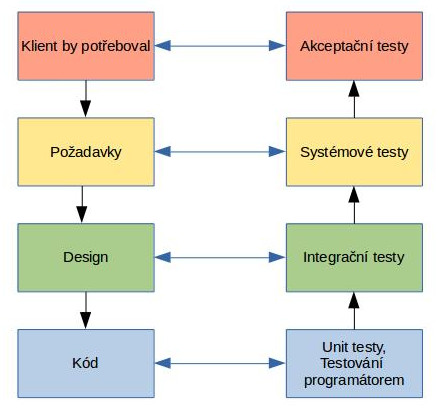
\includegraphics[width=.6\LW]{test_phase}
  \caption{Schéma testovacího modelu}
  \label{fig:test_phase}
\end{figure}

\subsection{Testování programátorem (Developer testing)}
První a úplně nezbytnou fázi testování by měli provádět programátoři. Programátor by si měl zkontrolovat jestli je možné firmware přeložit a dále jestli jeho nová či opravená funkcionalita funguje správně. V další fázi testování by měl zkontrolovat kód jiný programátor, který kód nepsal. Tuto fázi většinou provádí správce projektu při zařazování nové či upravené funkce do hlavní větve repozitáře projektu. Všechny chyby odchycené v této fázi testování ušetří spoustu času stráveném v dalších fázích testování.

Testování programátorem může vypadat jako samozřejmá věc, která by nemusela být ani uváděna. Bohužel opak je pravdou a i tato situace může nastat. V případě že je tato fáze vynechána je pravděpodobné že spousta chyb je odhaleno až ve fázi systémového testování, kdy zjišťování, reportování a oprava chyb stojí značnou režii.

\subsection{Testování jednotek (Unit testing)}
Úroveň testování jednotek obsahuje testování jednotlivých částí nebo modulů softwaru. Za jednotku neboli část lze považovat objekt s jednou jedinou funkcionalitou, a to například třídu, objekt, program či softwarový modul. Tato úroveň testování testuje správnost zdrojového kódu a ne funkci programu jako celku. Velmi známým příkladem jsou JUnit testy v javě, kde ke každé třídě a metodě je vytvářena testovací třída či metoda.

Unit testy je výhodné použít při tvorbě nového projektu, jelikož s unit testy je potřeba počítat již při návrhu zdrojového kódu a při návrhu kódu zároveň testy vytvářet. Dopisování testů do již existujícího projektu by stálo neúměrnou námahu a mnoho úprav kódu pro přizpůsobování samotného programu pro unit testování.

Zdrojový kód pro výrobky testované navrhovaným testovacím systémem je vyvíjen již 10 let a zároveň na těchto zdrojových kódech jsou stavěny i nové výrobky. Navíc přes devadesát procent firmwaru používá opensource řešení. Díky těmto dvěma skutečnostem je v nynější situaci nereálně přidat unit testování do navrhovaného testovacího schématu.

\subsection{Integrační testování (Integration testing)}
Po předchozích dvou úrovních testování, jenž jsou prováděny programátory, přichází fáze, kdy se hotový výrobek dostává do ruky testerům. Testeři většinou provádí dvě úrovně testování, integrační testování a systémové testování. Někdy jsou tyto dvě fáze spojovány do jedné a nazývají se systémově integrační testování. Obě úrovně budou dále detailněji popsány.

\begin{figure}[h]
  \centering
  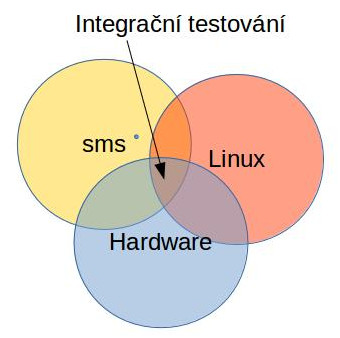
\includegraphics[width=.4\LW]{test_integration}
  \caption{Grafické znázornění integračního testování}
  \label{fig:test_integration}
\end{figure}

Pomocí integračního testování testujeme integraci jednotlivých komponent mezi ostatní komponenty, dále také integraci jednotlivých komponent do operačního systému, či na konkrétní hardware. Jako příklad mohu uvést testování integrace programu odesílání sms zpráv na operačním systému Linux, běžícím na hardwaru konkrétního routeru. Příklad znázorňuje, že není testováno pouze odesílání sms zpráv, ale komponenta v závislosti na operačním systému a hardwaru. Jednotlivé komponenty mohou být například subsystémy, databázové implementace, infrastruktura, rozhraní a systémové konfigurace. Integrační testování lze z testování vypustit, jelikož chyby nalezené v této fázi by byly odhaleny ve fázi systémového testování, nýbrž za cenu vyšší časové náročnosti.

Integrační testy navrhují testeři na základě čtyř základních skutečností a to softwárový a systémový design výrobku, architekturu firmwaru, pracovního postupu s danou komponentou a možnými případy použití. Na základě těchto čtyř skutečností tester navrhne testovací případy a postupy. Podle těchto postupů jsou jednotlivé komponenty dále testovány manuálně testery či automaticky automatem.

Testovací automat bude v prvním kroku testovat integračními testy všechny základní komponenty routeru, jako například posílání SMS zpráv, či SMPT klient vůči operačnímu systému Linux či uCLinux běžícím na každém z 50 různých výrobků podporujících testovanou funkcionalitu. Zde je nejlépe vidět přínos testovacího automatu. Ve skutečnosti by tester měl provést test integrace všech funkcionalit na všech padesáti odlišných výrobcích, což je časově značně náročné. Zatímco automat tento test může provést každý den na všech výrobcích paralelně během chvilky. Tímto testováním je ověřena integrace daného programu na všech výrobcích a neunikne žádná chyba způsobená chybou v firmwaru, či chybou některé ze součástí routeru, čímž může být například odlišná implementace odesílání sms v bezdrátovém modulu.

\subsection{SIT - Systémové testování (System testing)}
Systémové testování je poslední fází testování probíhající ve společnosti vyvíjecí daný produkt. Ve fázi systémového testování se testuje výrobek jako celek z pohledu zákazníka. Jsou navrhnuty jednotlivé testovací případy, které mohou nastat v praxi, a dle těchto případů jsou výrobky testovány. Příklad takového testovacího scénáře může být testovaný router do kterého je přes Ethernet připojena IP kamera a přes sériové rozhraní teplotní senzor. Data z těchto zařízení jsou přes OpenVPN tunel sestavený přes mobilní spojení posílána na vzdálený server.

\begin{figure}[h]
  \centering
  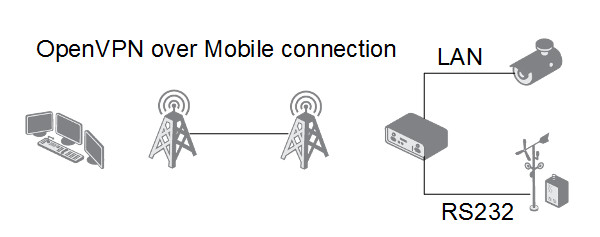
\includegraphics[width=.8\LW]{system_test_example}
  \caption{Příklad systémového testování}
  \label{fig:system_test_example}
\end{figure}

Systémové testy mohou obsahovat funkční i nefunkční testy, které jsou dále popsané v sekci věnované těmto typům testování. Dále je možné testovat kvalitu či rychlost přenosu dat, které mohou být prováděny na výrobcích ve standartním, ale i ve stiženém prostředí, například v klimatické komoře nebo v okolí EMC vyzařovaní. Na systémové testování je také možné pohlížet jako na testování bílé či černé skříňky. Oba způsoby jsou také dále popsány v kapitole věnující se dalším typům testování.

V navrhovaném případě testování bude systémové testování prováděno ve stejném kroku a pomocí stejných nástrojů jako integrační testování, čili tento model se blíží dříve zmíněné možnosti spojení systémových a integračních testů. V navrhovaném případě testování lze někdy určit hranici mezi systémovými a integračními testy a někdy je toto rozdělení obtížné určit. Většina systémových testů obdobně jako integrační testy bude možné provádět automaticky pomocí testovacího automatu. Jiné systémové testy, jako například testy v klimatické komoře, budou muset být dále z kapacitních důvodů prováděny manuálně, jelikož všech padesát výrobků se do klimatické komory nevejde. Naopak tyto testy nezávisí na změně firmwaru, čili ve většině případech stačí pouze jedno provedení klimatických testů při vyvinutí nového hardwaru výrobku a ne při každé změně firmwaru.

\subsection{UAT - Akceptační testování (Acceptance testing)}
Poslední úrovní testování je akceptační testování. Akceptační testování již není prováděno testery ve firmě, kde je výrobek vyvíjen. Testování je prováděno u cílového zákazníka na konkrétní aplikaci výrobku. Případné chyby či nesrovnalosti od požadované funkcionality jsou reportovány zpět a bývá očekávána rychlá reakce na opravu těchto chyb. Snaha testovacího systému samozřejmě bude odhalit všechny případné chyby před touto úrovní, tedy před dodáním výrobku zákazníkovy. Jelikož se tato fáze provádí až u koncového zákazníka, práce se touto fází dále nebude zabývat.

\section{Testovací procesy}
Fáze systémového a integračního testování lze provádět pomocí třech různých přístupů k testování. Všechny tři přístupy se od sebe liší hlavně v délce a složitosti návrhu testování a v délce samotného provádění testů. V neposlední řadě se liší jejich pokrytí testovacích případů a tím i kvalita testování. Podle složitosti návrhu testů by bylo možné popisované přístupy testování seřadit sestupně na testování založené na modelech, automatizované testování a poslední manuální testování. Rychlostí a efektivitou provádění testů jsou tyto způsoby seřazeny přesně opačně. Cílem této práce je automatizovat a tím zkrátit provádění testů a zároveň rozšířit možností testování. Z cíle práce tedy vyplývá, že se budu snažit pokusit o přechod z nynějšího manuálního testování na automatizované testování a v nejlepším případě na testování založené na modelech.

\subsection{Manuální testování}
Prvním přístupem provádění testů je manuální testování. Manuální testování je možné rozdělit do dvou nezávislých kroků. Prvním krokem každého manuálního testování je vytvoření testovacího plánu. Testovací plán obsahuje informace o tom, co by mělo být na výrobku testováno, jak by měl být výrobek testován a nakonec jak často by měl být výrobek testován. Dle tohoto plánů navrhuje testovací technik testovací scénáře a jejich jednotlivé testovací procedury. Navrhování testovacích procedur se provádí pokaždé při změně nebo přidání nějaké funkcionality výrobku. Návrh provádí testovací technik s požadovanými znalostmi o testovaném výrobku.

\begin{figure}[h]
  \centering
  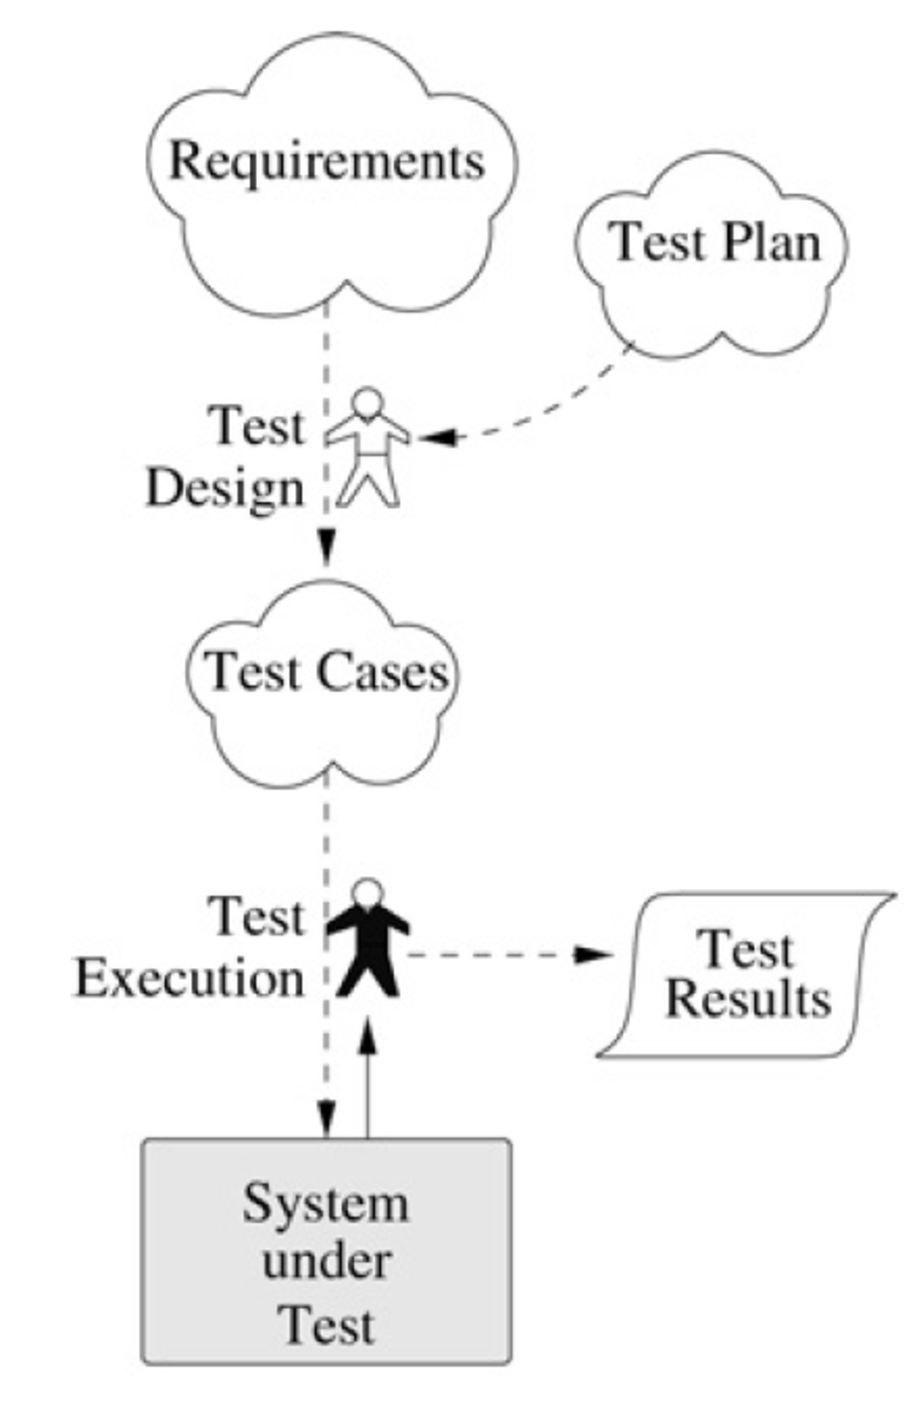
\includegraphics[width=.4\LW]{test_manual}
  \caption{Schéma manuálního testování}
  \label{fig:test_manual}
\end{figure}

Druhou fází manuálního testování je samotné provádění testů. Testy se provádějí manuálně přímo na testovaném objektu podle předepsaných testovacích procedur. Provádění testů je opakováno při každé změně ve firmwaru výrobku a dle jeho komplexnosti bývá i velice časově náročný. Z toho důvodu bývají některé testy vypouštěny, ale na úkor kvality testování celého výrobku. Samotné testování je práce manuální dle předepsaných pokynů a také velmi často se opakující, z toho plyne, že tuto práci může vykonávat tester bez znalostí návrhu testování samotných výrobků a jejich technologií. Dále se tento proces přímo nabízí k nějakému zlepšení jakoukoliv automatizací.

Ve společnosti, kde bude testovací systém nasazován, se nyní všechny testy provádějí manuálně dle předepsaných testovacích procedur. Jak už bylo v úvodu zmíněno, při rychle rostoucím počtu výrobků a jejich funkcionalit je nadále tento systém testování neudržitelný. Provádění integračních a systémových testů se budu snažit přesunout do jednoho ze sofistikovanějších způsobů testování. Dále pro specifické testy jako například EMC testy a klimatické testy v teplotní komoře nebude z kapacitních důvodů možné plně automatizovat a bude možné navrhnout moduly pro zjednodušené manuální testování.

Mohou nastávat i případy manuálního testování, kdy nejsou vytvořeny testovací plány a testovací procedury, kde možné později doložit adekvátní výsledky testování. Další nevýhodou tohoto přístupu k testování je vynechání velkého množství testovacích případů, jelikož se jedná spíše o náhodné testování, proto tento postup není určitě doporučován.

\subsection{Automatizované testování}
Druhým a sofistikovanějším způsobem provádění testů je automatizované testování, někdy také nazývané testování založené na skriptech. Automatizované testování lze rozdělit do třech základních fází. První fáze vytvoření testovacího plánu je shodná s manuálním testováním.

\begin{figure}[h]
  \centering
  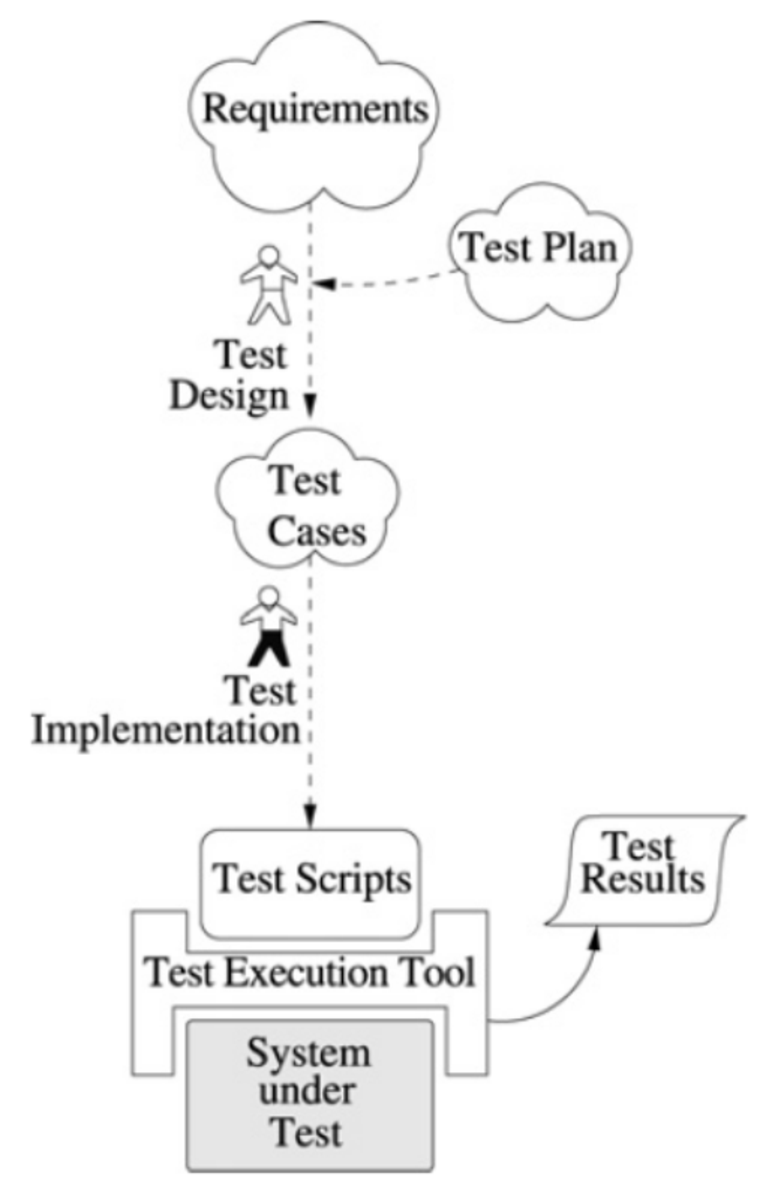
\includegraphics[width=.4\LW]{test_automat}
  \caption{Schéma automatického testování}
  \label{fig:test_automat}
\end{figure}

Druhou fází automatického testování je implementace testovacích procedur do spustitelných skriptů. Skriptovací testy mohou být napsány v nějakém standardním programovacím či skriptovacím jazyku nebo v jazyku přímo určenému k psaní testovacích skriptů. V našem systému bude k psaní testovacích skriptů použit skriptovací jazyk Bash a jednoduché programy napsané v programovací jazyk C. V automatizovaném přístupu testování nám přibyla další role programátora potřebného k implementaci testovacích procedur do spustitelných skriptů. Testovací skript je spustitelný skript nebo program, který provede jednu testovací proceduru. Testovací skript obvykle obsahuje inicializaci testovacího zařízení, uvedení testovacího zařízení do požadovaného kontextu, vytvoření vstupních testovacích hodnot, předání vstupních hodnot do testovaného zařízení, nahrání odpovědi od testovaného zařízení, nakonec porovnání odpovědi a očekávaného výstupu a vyhodnocení výsledku.

Třetí fází automatického testování je automatické spouštění testů. Testy jsou spouštěny automaticky pomocí nástroje pro spouštění testů. Nástroj provádí spouštění testů automaticky bez interakce s obsluhou. Nástroj navíc obsahuje možnost paralelizace testů nezávislých na nějakém zdroji. Zde je vidět veliká časová a tedy i finanční úspora oproti manuálnímu testování. Jestliže chceme provést nový test zařízení, spustíme pouze testovací nástroj a není potřeba manuálně testovat všechny funkcionality.

Naopak tento přístup přináší větší režii při změně funkcionality či přidání nového zařízení. Pokud je změněna testovací procedura či přímo funkcionalita výrobku, musí být předělány a přidány testovací skripty. Tato údržba může být v případech intenzivního vývoje stejně časově nákladná jako tvorba nových testovacích procedur pro danou funkcionalitu.

\subsection{Testování založené na modelech}
Nejsofistikovanějším řešením testování je testování založené na modelech, známé taky jako MBT (Model Base Testing). Zjednodušeně lze model tohoto systému popsat následovně. Tester vytvoří model testovaného zařízení, z tohoto modelu se automaticky vygenerují testovací skripty, které jsou spouštěny nad testovaným výrobkem. U tohoto testování odpadá spoustu času při návrhu a úpravách testovacích skriptů. Naproti tomu je velmi časově náročné navrhnutí samotného testovacího systému a modelu testovaného výrobku. Samozřejmě, že všechno není tak jednoduché, jak se na první pohled zdá a tak dále jsou detailně popsány všechny fáze tohoto způsobu testování. Jednotlivé fáze MBT jsou vývoj modelu testovaného zařízení, generování abstraktních testů z modelu, převedení abstraktních testů na spustitelné testy, spuštění testů na testovaném zařízení a analýza výsledků testů.

\begin{figure}[h]
  \centering
  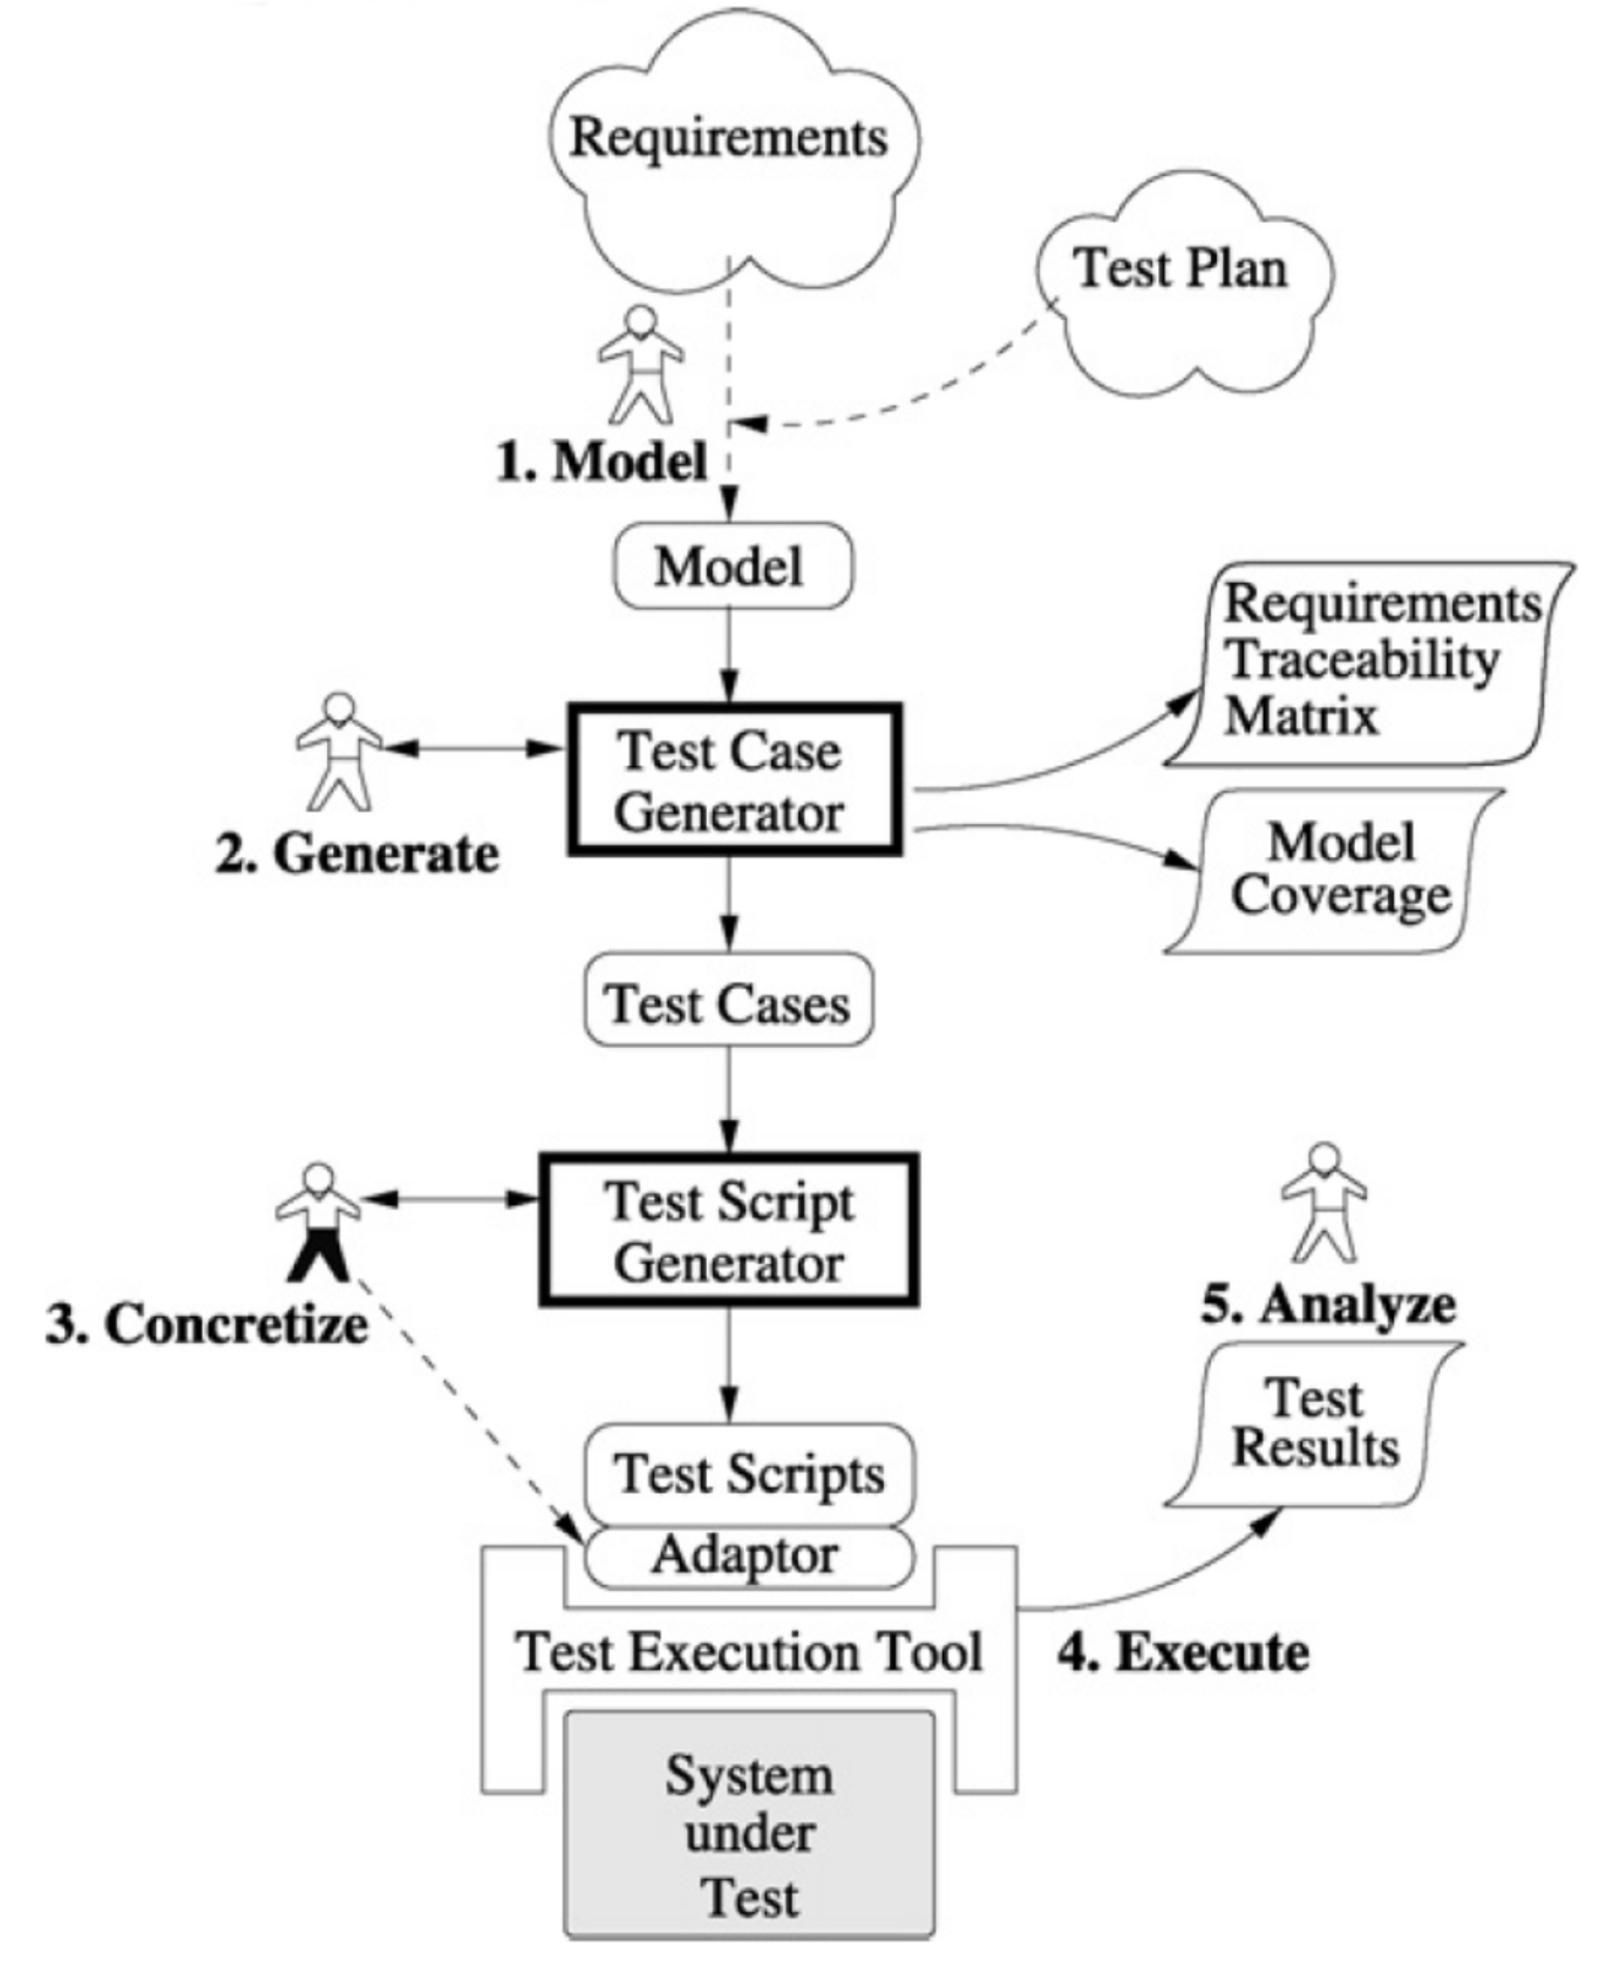
\includegraphics[width=.5\LW]{test_model}
  \caption{Schéma testování založeného na modelech}
  \label{fig:test_model}
\end{figure}

Prvním krokem testování založeném na modelech je tedy vytvoření abstraktního modelu testovaného zařízení. Model by měl být jednodušší nežli samotné zařízení a měl by se zaměřit na jeho klíčové vlastnosti.

Druhým krokem testování založeném na modelech je generování abstraktních testů z hotového modelu. Jelikož by ve většině případů bylo vygenerováno nekonečné množství testovacích případů, tak je potřeba určit nějaké testovací kritéria, aby bylo možné vygenerovat konečné množství testů. Tyto testy jsou sekvencí operací nad modelem. Používají zjednodušený pohled na testované zařízení a nejsou přímo spustitelné.

Třetí částí testování založeném na modelech je transformace abstraktních testů na spustitelné konkrétní testy. Transformace může být prováděna dvěma způsoby. Prvním způsobem je transformační nástroj, který používá šablony a mapuje každý abstraktní testovací případ do spustitelného skriptu. Nebo je možné napsat adaptér kódu, který implementuje každou abstraktní operaci jako operaci nad testovaném zařízení a doplní jí detaily, které nejsou navrženy v abstraktním modelu.

Ve čtvrtém kroku jsou spouštěny konkrétní testy na testovaném systému. Tato fáze je shodná s třetí fází automatizovaného testování. Tedy může používat stejný systém a ve zjednodušené variantě lze říci, že jde pouze o jiné generování testovacích skriptů. Dále jde tento krok rozdělit na online a offline testování. Při online testování se generují testy při každém spuštění testu. Při offline testování jsou testy předem generovány a pokud nenastane změna v testovacím modelu, jsou používány stejné již předem generované testy.

V posledním pátém kroku se analyzují výsledky spuštěných testů a jejich korektní chování. V případě neúspěšného kroku se analyzuje příčina a místo vzniku chyby. Nejčastější místa vzniku chyby jsou chybný model, chybný adaptér kódu a v neposlední řadě může chyba vzniknout chybnou funkcí testovaného výrobku.

Z popisu tohoto způsobu testování je vidět, že v případě správné implementace tohoto systému na testovaný produkt by mohlo výrazně usnadnit práci při testování. Samotná implementace je velmi složitá a ne všechny testované objekty lze efektivně popsat tímto systémem. Nasazení systému testování založeného na modelech ztroskotalo po několika letech i ve velkých společnostech jako například IBM. V testovacím systému pro výrobky společnosti Conel bude snaha použít systém testování založeného na modelech alespoň  na  nevyšší abstraktní úrovni.

\section{Typy testování}
Poslední podkapitola typy testů probírá pojmy z testování, které nebyly obsaženy v žádném z předchozích modelů a v testování se občas používají či naopak je některý z předchozí modelů používá a nebyly detailně popsány.

\subsection{Testy splněním a selháním}
Testy splněním používají vstupní data pouze množinu dat, které testovaný systém musí správně vyhodnotit, taktéž se chováme k systému korektním způsobem, při tom kontrolujeme jestli odpověď od testovaného systému se shoduje s očekávanou odpovědí. Naopak při testech selháním zacházíme s testovaným systémem nekorektně a na vstup mu přivádíme data, které systém neumí vyhodnotit a kontrolujeme jestli systém nespadl či systém nevrací odpověď shodující se s očekávaným výstupem.

\subsection{Progresní a regresní testy}
Progresními testy nazýváme testy kontrolující nové funkce testovaného výrobku. K sestavení progresních testů je nutná znalost nových funkcí daného výrobku. Regresními testy se nazývá opětovné testování již testovaných vlastností výrobků. Regresní testy jsou často prováděny při dokončení části vývoje pro ujištění, zda-li nové úpravy neovlivňují jiné části firmwaru. Taktéž jsou prováděny před vydáním nového firmwaru.

\subsection{Smoke testy}
Smoke testy je označení testů obsahující pouze jednoduché testování spustitelnosti produktu a jeho základních funkcionalit. Většinou se toto testování provádí před systémovými testy. Největší význam těchto testů přichází ve výrobě nových produktů pro ověření funkčnosti vyrobeného výrobků.

\subsection{Funkční a nefunkční testy}
Pomocí funkčních testů jsou testovány všechny funkce implementované v testovaném výrobku a jejich správné fungování. Tyto testy jsou popisovány v předchozích kapitolách. Další metodou jsou často opomíjené nefunkční testy testující funkce výrobku přímo nesouvisející s jeho funkcionalitou. Jedná se například o testování výkonu celého výrobku nebo jeho částí. Kontroluje se zde jestli výrobek dosahuje požadovaného výkonu a zároveň jestli je při zvýšené zátěži stále dobře funkční.

\subsection{Testování bílé a černé skříňky}
Testování bílé skříňky je prováděno, pokud při navrhování testů má tester přístup a využívá zdrojových kódu testovaného výrobku. Naopak při testování černé skříňky tester zdrojové kódy k dispozici nemá a k návrhu testů využívá pouze dokumentace k danému výrobku.

\subsection{Statické a dynamické testy}
Statické testy nepotřebují ke svému provádění spuštěný program. Naopak dynamické testy ke svému fungování potřebují spuštěný funkční program.

\endinput

  \chapter{Dostupné testovací nástroje}
V kapitole dostupné testovací nástroje popíšu zkoumanou část dostupných opensource i komerčních nástrojů pro jednotlivé fáze testování. U všech testovacích nástrojů bude posuzován přínos v případě nasazení v testovacím systému pro výrobky společnosti Conel.

\section{Jenkins CI}
Jenkins CI je nástroj pro kontinuální integraci. Kontinuální integrace spočívá v častém kompilování zdrojového kódu a následném spouštění testů nad tímto softwarem.
Jenkins CI je nástroj napsaný v programovacím jazyce Java. Tento nástroj má podporu  kompilace různých projektů díky veliké možnosti nastavení a velké podpoře v podobě rozšiřujících pluginů, jejichž počet neustále roste.

\begin{figure}[h]
  \centering
  
\includegraphics[width=.3\LW]{jenkins_logo}
  \caption{Logo produktu http://www.jenkins-ci.org}
  \label{fig:testlink_logo}
\end{figure}

Jenkinsen je dobrý a přehledný buildovací systém s podporou mnoha programovacích jazyků. Velikou výhodou tohoto systému je opensource řešení projektu, naopak nevýhodou jsou veliké systémové požadavky nástroje. Tento systém sice podporuje testování, ale podporuje pouze testování na úrovní testování jednotek, které v navrhovaném systému nebude vůbec využito. Jenkins CI naopak nepodporuje funkční a systémové testování na konkrétním hardwaru, které je v testovacím systému vyžadováno.

\begin{figure}[h]
  \centering
  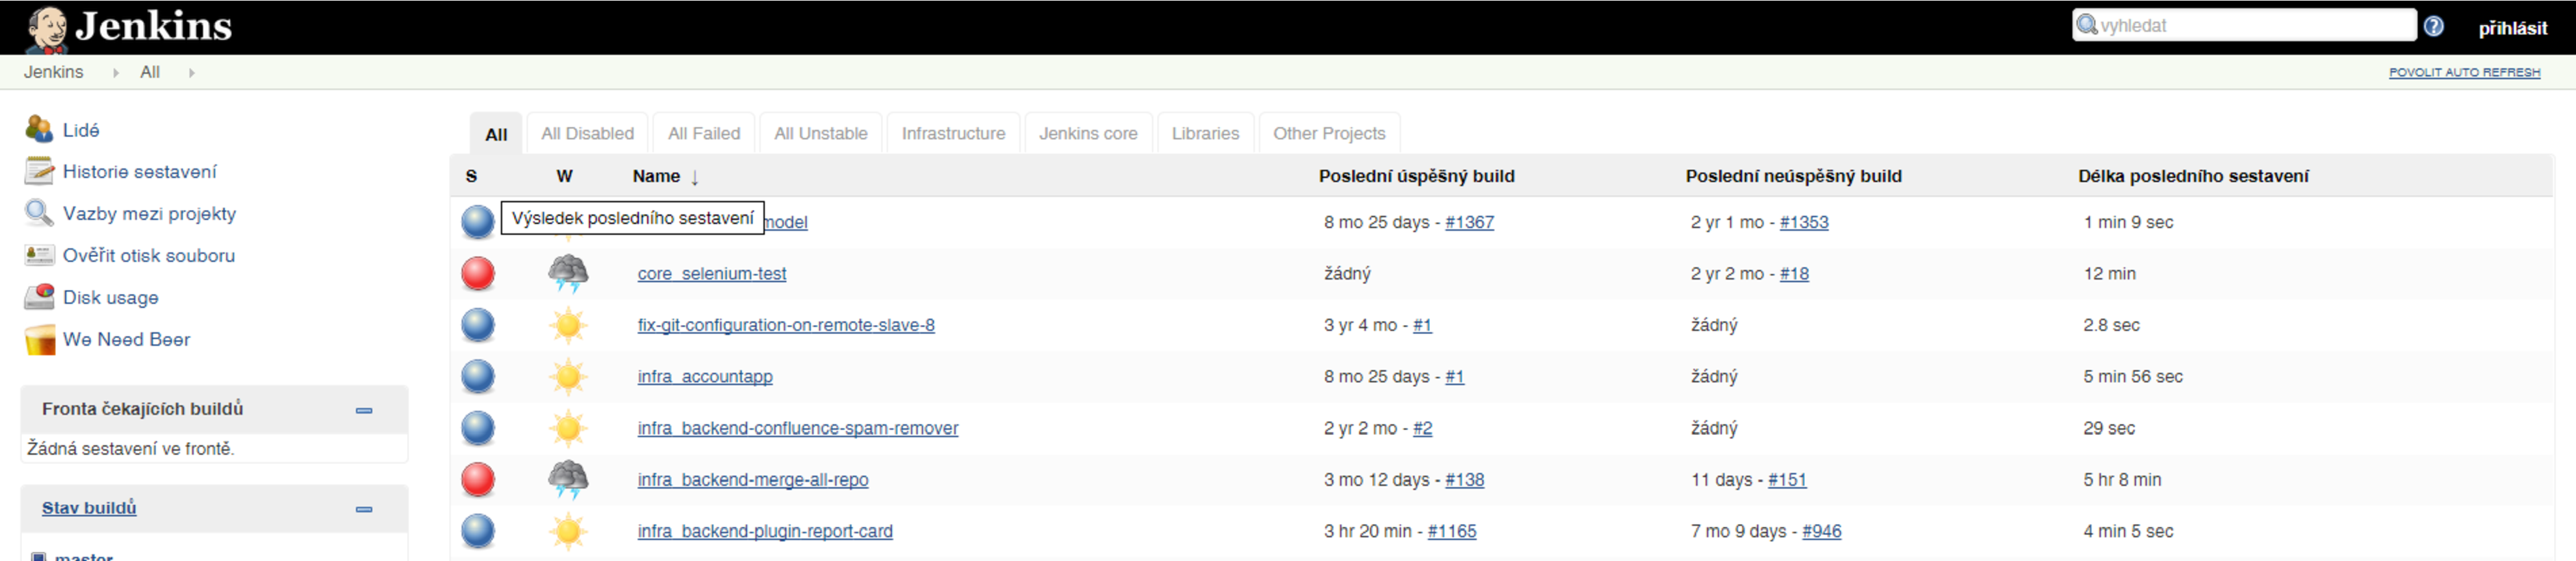
\includegraphics[width=\LW]{jenkins_example}
  \caption{Příklad otevřené aplikace Jenkinsen}
  \label{fig:testlink_example}
\end{figure}

Použití nástroje Jenkins CI pro kontinuální integraci v testovacím zařízení by bylo možné pouze ve fázi buildování všech firmwarů. Skripty zajišťující správnou funkci s buildovacím program ltib je potřeba napsat stejné jak při použití systému Jenkins, tak při vlastním spouštění překladu. LTIB je image systém používající se pro překlad většiny testovaných výrobků. Taktéž samotné spouštění těchto skriptů bude v testovacím systému již implementováno v části obsluhující spouštění testovacích skriptů. Na základě těchto skutečností jsem upřednostnil použití vlastního spouštění kompilačních skriptů, hlavně z důvodu jednotného systému pro vizualizaci všech informací o průběhu všech fází překladu a testování.

\section{Testlink}
Testlink je nástroj pro správu a organizaci testů. Nástroj je vytvořený jako webová aplikace napsaná v jazyce PHP využívající databázi MySQL nebo PostgeSQL. Aplikace je zdarma i pro komerční účely, jelikož je šiřená pod licencí GPL.

\begin{figure}[h]
  \centering
  
\includegraphics[width=.3\LW]{testlink_logo}
  \caption{Logo produktu http://www.testlink.org}
  \label{fig:testlink_logo}
\end{figure}

Nástroj testlink umí spravovat a organizovat testy a testovací případy. Testlink obsahuje pět základních pilířů, o které se dále opírá a tvoří jeho strukturu. Prvním a základním prvkem je testovací případ neboli test case. Testovací případlze přirovnat k skriptu či testovací proceduře popisované ve způsobech testování. Dalším prvkem je sada testů označovaná test suite. Sada testů organizuje testy do funkčních skupin. Třetím prvkem nástroje testlink je testovací plán. Testovací plán je sestaven ze sad testů a dále z dalších informací o daném testování. Dalším prvkem je testovací projekt, který je základním prvkem systému. Testovací projekt v známé terminologii odpovídá testovanému subjektu. Posledním prvkem tohoto systému je uživatel. Jednotlivý uživatelé mají různá práva úprav v systému, aby byla zavedena bezpečnost systému. Tento systém umí také podle vložených výsledků testů vytvářet reporty o testování v různých formátech.

\begin{figure}[h]
  \centering
  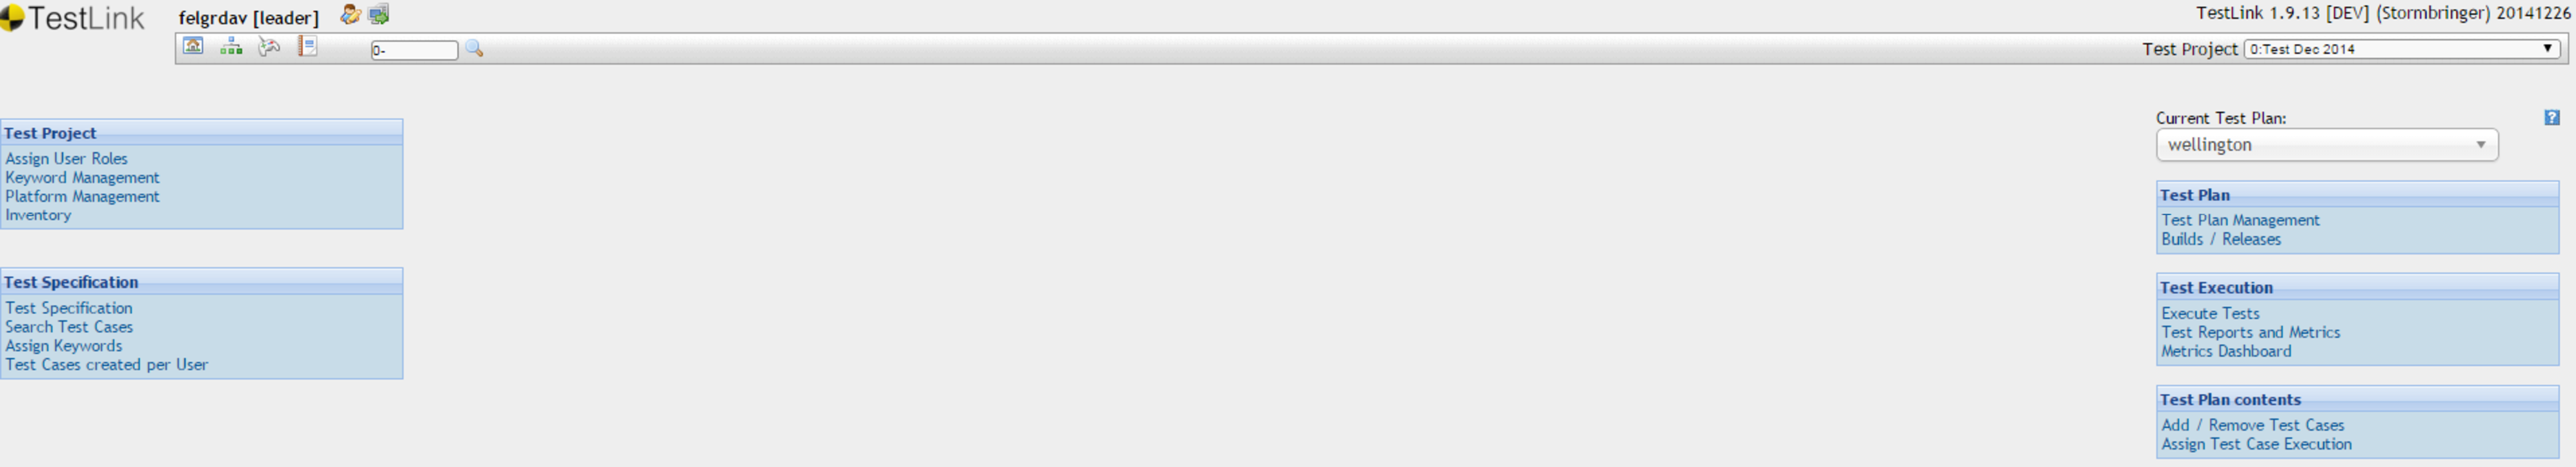
\includegraphics[width=\LW]{testlink_example}
  \caption{Příklad otevřené aplikace Testlink}
  \label{fig:testlink_example}
\end{figure}

Nástroj Testlink může být účinný v případě manuálního testování pro snadnou správu testů a reportování výsledků těchto testů. I v případě navrhovaném testovacím systému společnosti Conel by bylo možné systém nasadit. Jestliže by byl systém nasazen, byly by nutné úpravy tohoto systém k požadavkům automatického testování a speciálním požadavkům na modulárnost testovaných výrobků. Po krátkém zkoumání jsem zjistil, že úpravy pro automatické testování a úpravy k potřebám hierarchie  testovací laboratoře by byli rozsáhlé. Dále systém Testlink působí velmi nepřehledně. Díky těmto závěrům bylo rozhodnuto nepoužití nástroje Testlink pro spravování testů a reportování výsledků.

\section{Selenium}
Selenium je nástroj pro testování webových aplikací. Nástroj Selenium je také opensource projekt napsaný v jazyce Java. Selenium je dostupné ve čtyřech variantách a to Selenium IDE, Selenium RC, Selenium WebDriver a Selenium Grid. Selenium IDE je plugin do internetového prohlížeče Firefox. Dále Selenium RC, který si sám pouští internetové prohlížeče a provádí na nich testy. Testy je možné psát v jazycích Java, C, Python, Ruby, Perl, PHP a pro psaní těchto testů je připraveno přehledné API. Seleneium WebDriver usnadňuje psaní samotných testů na úkor nutnosti psaní všech testů na každý prohlížeč. Poslední Selenium Grid umožňuje paralélní spouštění testů na více strojích i počítačích.

\begin{figure}[h]
  \centering
  
\includegraphics[width=.1\LW]{selenium_logo}
  \caption{Logo produktu http://www.seleniumhq.org}
  \label{fig:selenium_logo}
\end{figure}

Selenium je dobrý nástroj pro testování webových aplikací. Nástroj bude určitě využitelný i pro testování webového rozhraní zařízeních testovaných v testovací laboratoři. V první fázi nasazení testovací laboratoře budou jednotlivé konfigurace měněni pomocí ssh a telnet přístupu do routeru. Jelikož tento nástroj více možností nepodporuje, tak nebude v první fázi nasazování testovacího zařízení využit.

\section{VectorCAST}
Nejlepším zkoumaným testovacím nástrojem byl komerční produkt VectorCAST od společnosti VECTOR Software. VectorCAST je platforma přímo určená k testování embedded zařízení podporující velkou škálu zařízení a testů.

\begin{figure}[h]
  \centering
  
\includegraphics[width=.4\LW]{vector_logo}
  \caption{Logo produktu http://www.vectorcast.com/}
  \label{fig:vector_logo}
\end{figure}

Samotný produkt je rozdělen do několika částí, které jsou dodávány zvlášť podle potřeb zákazníku a typu cílové testované aplikace. První dva programy se zabývají testováním jednotek a integračním testováním. První program je VevtorCAST/Ada, který je určen pro testování softwaru napsaném v jazyce Ada. Ada je robustní staticky typovaný programovací jazyk určený pro programování kritických aplikací. Tento jazyk v testovaných zařízeních nikdy nebyl použit a tak se dále tímto programem nebudu zabývat. Druhým programem určeným pro testování jednotek a integrační testování je VectorCAST/C++ určeným pro aplikace psané v jazycích C a C++.

VectorCAST/C++ je řešení pro automatizované testování jednotek a integrační testování. Tento nástroj přímo automatizuje vytváření unit testů pro samotný zdrojový kód. Nástroj je možné spustit nativně nebo na konkrétní cílové platformě. Pro spouštění na cílové platformě je potřeba nástroj VectorCAST/RSP, který bude popsán později. Další vlastností tohoto systému je jednoduché regresní testování softwaru, kdy je možné automaticky spouštět již vytvořené testy. Nástroj může pracovat ve dvou módech a to Source mód a Agile mód. První Source mód tvoří testy z modulů, které jsou již implementovány. Druhý Agile mód nepotřebuje pro tvorbu testů zdrojové kódy daného modulu, ale stačí mu pouze jeho hlavičkové soubory.

\begin{figure}[h]
  \centering
  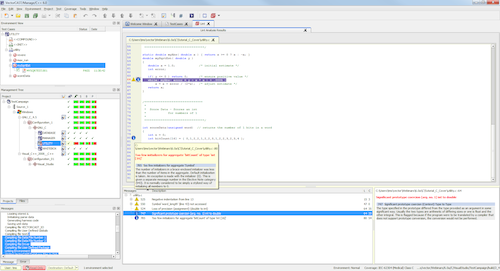
\includegraphics[width=\LW]{vector_example}
  \caption{Příklad otevřené aplikace VectorCast}
  \label{fig:vector_example}
\end{figure}

Pro lepší správu regresního testování slouží nástroj VectorCAST/Manage. Nástroj je vhodný pro vývoj aplikací s dlouhým životním cyklem, či s většími vývojovými týmy. Členové celého týmu mohou pohodlně spouštět regresní testy a sledovat jejich výsledky. Nástroj dále obsahuje podporu testování aplikace na více operačních systémech, více cílových platformách a různých konfiguracích. Testování stejného modelového případu ve všech možných situacích je důležité pro stoprocentní ověření systému. Nástroj umožňuje také funkci testování založené na změnách, kdy nástroj sleduje změny zdrojový kódů a spouští pouze testy modulů na kterých byli provedeny změny.

VectorCAST/Cover analyzuje využití kódu v průběhu systémového testování. Pomocí tohoto nástroje je možné zjistit, jaká část aplikace nebyla při samotném systémovém testování testována. Druhým nástrojem pro analýzu kódu VectorCAST/MCDC můžeme provést analýzu všech možných stavů a podstavů kam se aplikace psaná v jazyk C či C++ může dostat.

Testované aplikace je možné testovat přímo na cílové platformě pomocí již dříve zmíněného nástroj VectorCAST/RSP. V tomto nástroji je implementována široká škála kompilátorů. Pomocí VectorCAST/RSP lze stáhnout testovací postup přímo na cílovou platformu, kde jsou všechny testy prováděny a výsledky odeslány zpět testovacímu zařízení. Všechny kroky probíhají automaticky na pozadí bez interaktivity obsluhy.

Řešení pro testování embbeded aplikací VectorCAST a jeho všechny doplňující balíky jsou velmi silným nástrojem. Po detailní zkoumání tohoto nástroje a jeho funkcionalit nemohu ani tento nástroj doporučit pro účely automatické testování výrobků společnosti Conel. Hlavním důvodem nevhodnosti použití tohoto nástroje je potřeba zdrojového kódu k tvorbě jak testování jednotek, tak integračního testování. Firmware v testovaných výrobcích je z devadesáti procent tvořen opensource projekty. Tvorba takových testů na veškerém software by byla velmi dlouhá práce s nejasným výsledkem, taktéž projekt neobsahuje žádnou podporu systémového testování a návrh testů vzhledem k modulárnosti testovaných zařízení.

\section{Maveryx}
Maveryx je komerční řešení pro automatizované testování aplikací s grafickým uživatelským rozhraním. Tato aplikace podporuje testování aplikací napsaných v jazyce Java a aplikací pro operační systém Android. Aplikace Maveryx se nebude hodit k použití v testovacímu systému, ani pro řešení žádného mezikroku testování.

\section{Robot Framework}
Robot Framework je framework pro automatizované akceptační testování a vývoj řízený testy. Základní testovací možnosti lze rozšířit pomocí nových knihoven napsaných v jazyce Java nebo Python, pomocí kterých je možnost doplňovat nová klíčová slova.

\begin{figure}[h]
  \centering
  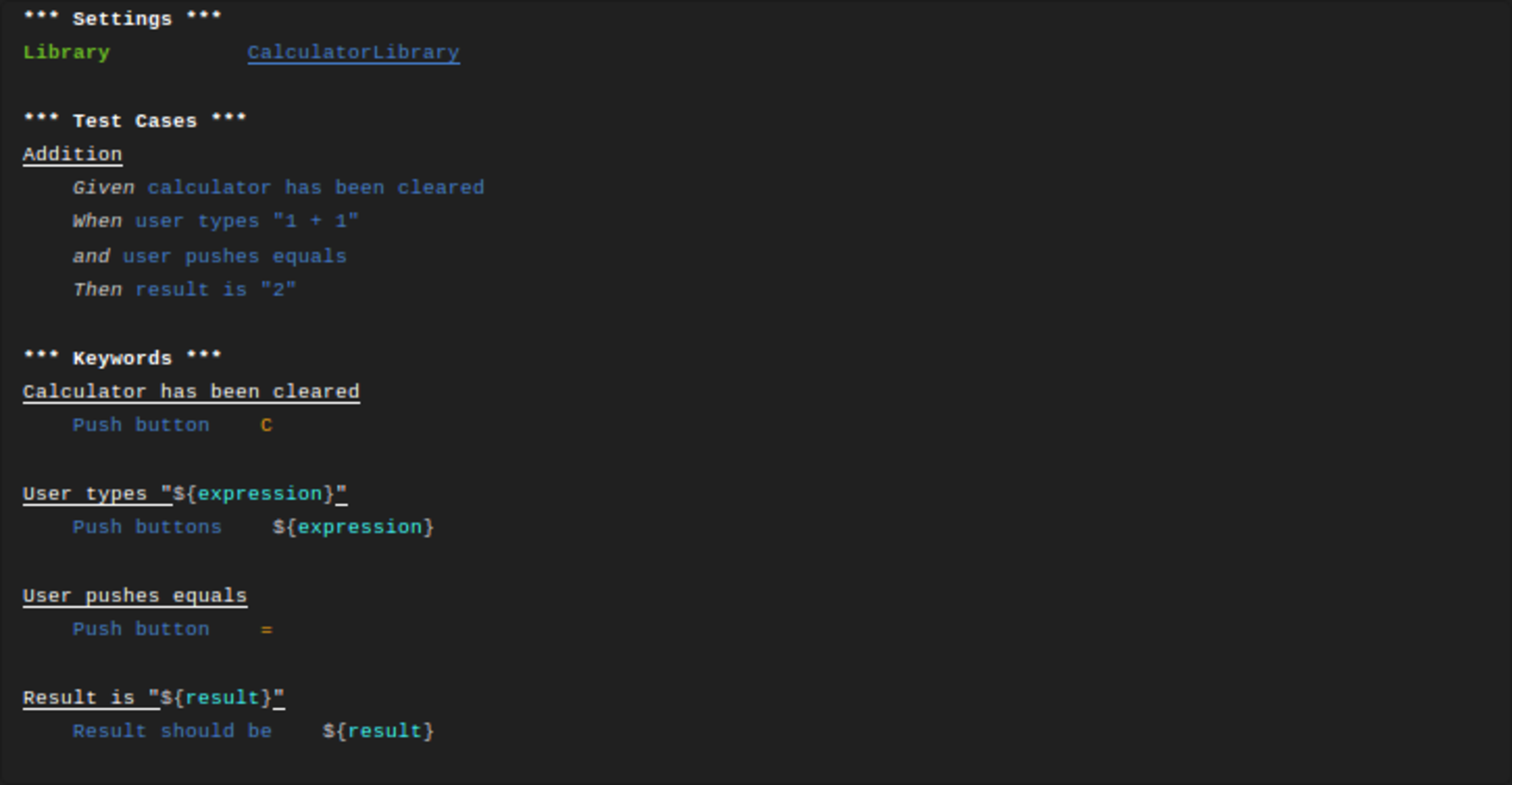
\includegraphics[width=\LW]{robot_example}
  \caption{Příklad testu ve framewotku http://robotframework.org/}
  \label{fig:robot_example}
\end{figure}

Robot Framework je pěkný příklad jak by mohl testovací framework vypadat. Specifické požadavky testovacího frameworku pro testování síťových embedded zařízení tento framework neobsahuje. Samozřejmě by se dali všechny knihovny dopsat pomocí přídavných knihoven a systém upravit k potřebám testovacího zařízení. Jednodušší cestou bude vzít dobré zkušenosti z testování tohoto frameworku a postavit vlastní API vhodné pro testování embedded aplikací.

Robot Framework je opensource projekt pod Apache Licencí 2.0. Robot Framework je nezávislý na operačním systému a aplikacích, jelikož jádro frameworku používá Python.

\section{Embedded Unit}
Embedded Unit je nástroj pro testování na úrovni testování jednotek. Nástroj je určen pro testování softwaru pro embedded aplikace. Jelikož tuto úroveň testování nebudu prozatím implementovat do testovacího systému, tak nebude tento nástroj prozatím využit.

\section{Linux Test Project}
Linux Test Project má za cíl testování stability, spolehlivosti a robustnosti Linuxového jádra a souvisejících funkcí. Tímto nástrojem bychom mohl testovat Linuxovou distribuci pro architekturu testovaných zařízení. S takto detailními testy se pro testovací laboratoř prozatím nepočítá, ale pro kvalitní testování výrobků se bude do budoucna hodit.

\section{Ostatní aplikace}
API pro vytváření jednotlivých testů bude využívat různé, převážně opensource programy ze světa síťových technologií. Například Curl pro komunikaci mnoha síťovými protokoly Všechny tyto použité programy budou popsány v kapitole věnující se API testovacího systému.

\endinput

  \chapter{Návrh testovací laboratoře}

Pro testování všech výrobků společnosti Conel nejdříve navrhnu strukturu testovací laboratoře.  Testovací laboratoř bude síť obsahující všechny výrobky společnosti Conel, různá příslušenství připojené k jednotlivým výrobkům, testovací server a konfigurovatelné switche.

\section{Testovací server}
Jádrem testovací laboratoře bude server na kterém poběží všechny testovací aplikace. Testovaci server bude výkonější počítač s parametry procesor Intel core i7, 16GB RAM a 512GB SSD disk. Pro účely testování bude server osazen dvěma ethernetovými rozhranímy pro komunikaci s testovanými výrobky a jedním ethernetovým rozhraním pro konektivitu serveru do firemní sítě. Server dále má osazeno jedno WiFi rozhraní pro testování WiFi výrobků.  Operační systém tohoto serveru jsem zvolil Ubuntu server, jelikož operační systém Ubuntu je používán k vývoji většiny výrobků.

\section{Konfigurovatelné switche}
Pro propojení všech výrobků s testovacím serverem budou použity dva konfigurovatelné 48 portové switche od firmy CISCO. Dva switche byly zvoleny kvůli velké ceně switchů nad 48 portů. Konfigurovatelné switch budou potřeba pro změnu síťové infrastruktury v průběhu testu. Každý switch bude připojen k jednomu ethernetovému rozhraní serveru, dále budou switche navzájem propojeny. Nejen všechny výrobky, ale každé fyzické ethernetové rozhraní bude připojeno do switche a pomocí VLAN bude vytvořena požadovaná testovací síť.

\section{Výrobky společnosti Conel}
Zařízení které tvoří přes devadesát procent prodeje firmy Conel jsou bezdrátové routery a i tato zařízení budou testovány v testovací laboratoři. Bezdrátové routery tvoří celkem čtyři modelové řady, které dále obsahují jednotlivé výrobky podle technologie bezdrátového připojení a počtu rozhraní.

\subsection{Řada routerů v0}
Takzvaná nultá řada routerů obsahuje pouze dvá výrobky. Prvním ER75i disponující EDGE technologií, jedním ethernet rozhraním možností a osazením jednoho volitelného portu.  Druhým výrobkem této řady je UR5, který se liší pouze bezdrátovou technologií. Místo EDGE technologie disponuje rychlejší UMTS technologií. Oba tyto výrobky jsou postaveny na uClinuxu a i přes jejich stáří se firmware stále udržuje.

\subsection{Řada routerů v1}


\subsection{Řada routerů v2}
\subsection{Řada routerů v3}

\section{Volitelné porty}
\subsection{Port LAN}
\subsection{Port WiFi}
\subsection{Port RS232}
\subsection{Port RS485/422}
\subsection{Port CNT}

\section{Cisco router}




\endinput

  \chapter{Pohled na modelové testování}
Po sestavení všech požadavků na testování výrobků a na samotnou testovací laboratoř byl navržen způsob implementace testování založeného na modelech. V první fázi nasazování tohoto způsobu testování na produkty společnosti Conel bude uvažováno pouze systémové testování všech testovaných zařízení. Modely budou vytvářeny na největší abstraktní míře a to na úrovni jednotlivých funkcí. Zjednodušeně popsáno má každé zařízení definováno svůj model, který nadefinuje správce testovacího zařízení. Každému modelu jsou přiřazeny vlastnosti zařízení a jednotlivé funkce, které by mělo modelované zařízení podporovat. Každá funkce obsahuje sadu spustitelných testovacích procedur, pomocí kterých je skutečné zařízení testováno. Na závěr celého testování se porovnává výsledek spouštěných procedur na skutečných zařízeních s výsledkem testu funkce na modelu zařízení. Na každém zařízení jsou spouštěny testy pouze funkcí, které podporuje model testovaného zařízení. Porovnání provádějí testovací skripty jednotlivých funkcí na základě vlastností modelu, zjištěných z databáze a na základě vlastností testovaného zařízení, zjištěných z připojeného testovaného zařízení.

\begin{figure}[h]
  \centering
  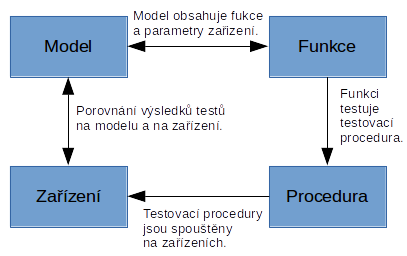
\includegraphics[width=.6\LW]{model_view}
  \caption{Pohled na modelové testování}
  \label{fig:model_view}
\end{figure}

\section{Funkce zařízení}
Základním pojmem tohoto přístupu bude funkce, kterou dané zařízení může podporovat. Každá funkcionalita jakéhokoliv testovaného zařízení je popsána právě touto základní vlastností. Příkladem takové funkce může být posílání sms zpráv. Každý router vlastnící bezdrátový modul umožňující tuto funkcionalitu bude tuto funkci poskytovat a naopak router bez bezdrátového modulu zřejmě tuto funkcionalitu nebude podporovat.

Funkce definuje vlastnosti chování dané funkcionality zařízení, způsob testování a předpokládaný výsledek testu na modelu. Dále je možné definovat hierarchii funkcí, aby nebylo možné testovat nějakou funkci bez předchozího úspěšného testu jiné funkce. Například nemá smysl testovat nahrání nového firmwaru do výrobku, pokud se nepovede úspěšně přeložit nový firmware.

\begin{figure}[h]
  \centering
  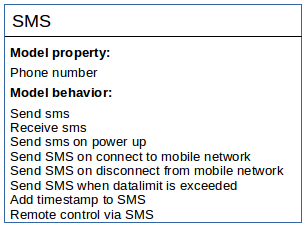
\includegraphics[width=.5\LW]{model_sms}
  \caption{Příklad funkce posílání sms zpráv}
  \label{fig:model_sms}
\end{figure}

\section{Testovací procedury}
Testování každé funkce bude prakticky realizováno pomocí testovací procedury. Každé funkci je přiřazena sada testovacích procedur, pomocí kterých jsou testovány všechny možné funkcionality dané funkce.

Testovací procedury jsou implementovány jako spustitelné skripty. Skripty jsou psány v jazyce BASH a pomocí testovacího API. Spouštěnému skriptu se jako paramtr předává identifikační číslo testovaného modelu a identifikační číslo testovaného releasu firmwaru. Skript spouští testy na daném routeru a porovnává výsledky testů spuštěném na routeru s výsledky testů spouštěných na modelu testovaného zařízení.

Praktické připojení na konkrétní zařízení je realizováno pomocí telnet či SSH spojení. Tento princip nám umožňuje testovat jakékoliv zařízení umožňující komunikaci jedním z těchto protokolů. Dále je možné přidání dalších protokolů, ale u navrhované testovací aplikace si vystačím pouze s těmito protokoly. Připojení na model zařízení je realizováno pomocí databáze, kde jsou uložena data modelu. Pro přístup k modelu i testovanému zařízení slouží řada programů z testovacího API, jenž jsou popsány v samostatné kapitole.

\section{Model zařízení}
Každému výrobku je ve webovém rozhraní vytvořen model. Model obsahuje informace o daném výrobku jako je název testovaného výrobku, číslo portu, do kterého je výrobek zapojen, IP adresu primárního portu výrobku a výchozí protokol komunikace se zařízením a další informace o tomto výrobku. Dále jsou tomuto modelu přiřazeny funkce, které daný model podporuje. Každý testovaný výrobek má tedy k sobě přiřazen model obsahující informace o tomto výrobku a množinu funkcí, jenž daný výrobek podporuje a mají být na něm testovány.

Při testování výrobků testovací program testlab dle parametrů modelu naváže s testovanými výrobky spojení. Po úspěšném navázaní spojení program spouští na daném zařízení testy definované v samotném modelu výrobku. Dále po provedení každého testu program porovnává výsledky testů spuštěných na testovaném zařízení s očekávanými výsledky testů spuštěných na modelu testovaného zařízení. Výsledky testů a případné chybové hlášky program zapisuje do databáze pro možnost vytvoření reportu z každého testování.

\section{Příklad modelu zařízení}
Pro snadnější pochopení implementace přístupu testování založené na modelech bude uveden příklad postupu vytváření modelu nového testovaného zařízení a jeho následné testování. Po ukončení základního vývoje je zařízení připojeno do testovací laboratoře. V dalším kroku je potřeba vytvořit model zařízení v testovací aplikaci. Model daného zařízení je vytvořen pomocí webové aplikace, jenž bude detailně popsána v kapitole věnující se webovému rozhraní testovací aplikace. Při vytváření modelu zařízení zadáme jeho parametry. Dále vytvořenému modelu přiřadíme funkce, které testované zařízení podporuje. Tímto krokem je ukončeno přidávání nového výrobku do automatického testování.

Pokud je model výrobku úspěšně přidán do testovacího zařízení, tak v dalším spuštění testování je nový výrobek již testován. Testovací program se připojí k testovanému zařízení a podle modelu spouští na testovaném zařízení jednotlivé testy a výsledky porovnává s výsledky testů provedených na modelu.

Konkrétním případem může být router LR77 v2F RS232, což je bezdrátový LTE router s volitelným sériovým rozhraním. Tomuto routeru přiřadíme IP adresu na primárním LAN interfacu 10.40.28.32, připojíme ho do třináctého portu switche. Výrobek podporuje komunikaci protokolem SSH i telnet a jako výchozí vybereme SSH protokol. Dále jsou  routeru přiřazený následující funkce. SSH připojení a telnet připojení jsou funkce potřebné k připojení k routeru, pokud tedy testování těchto funkcí skončí úspěšně pokračuje se na testování dalších funkcionalit routeru. Nyní je testován spojení do mobilní sítě ppp, jestliže je router úspěšně připojen je možné testovat Up/Down skripty routeru a zálohované připojení VRRP. Dále nezávisle na ppp spojení je testována funkcionalita sms zpráv a sériového rozhraní RS232.

\begin{figure}[h]
  \centering
  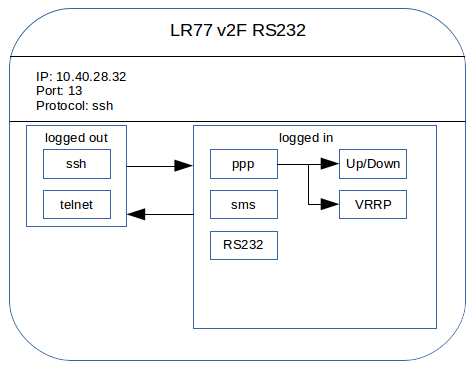
\includegraphics[width=.5\LW]{model_LR77}
  \caption{Příklad modelu routeru LR77 v2F RS232}
  \label{fig:model_LR77}
\end{figure}

\section{Výhody modelového přístupu}
Díky tomuto přístupu není potřeba při přidávání nového výrobku psát nové testovací skripty pro testování výrobku, ale pouze navolíme vlastnosti výrobku. Výrobek je testován dle testovacích procedur navolených funkcí. Pokud je vyvinuta nová funkcionalita, jsou pro tuto funkcionalitu napsány testovací skripty a všem zařízením podporujícím tuto funkcionalitu se pouze přidá nová funkce v jejich modelu a dále není potřeba psát testovací procedury pro všechny možné routery zvlášť. Pokud dojde ke změně zapojení v testovací laboratoři, opět není nutné přepisování všech testovacích skriptů routerů, kterých se tato změna týká, ale pouze je změněn model zařízení a testování funguje dále beze změn.

\endinput

  \chapter{Testovací program}
Testovací systém běžící na serveru testovací laboratoře se skládá z několika samostaných částí. Základem celého systému je databáze uchovávající všechna informace struktuře testovací laboratoře, informace o všech modelech testovaných zařízení, data s výsledky jednotlivých testů. Program testlab jenž se stará o celý průběh testování. Několika málo přepínači lze nastavit průběh testování. Další součástí je sada programů nazývající se testovací API. Tyto programu usnadňují psaní jednotlivých testů. Nedílnou součástí testovacího systému jsou testovací skripty, které lze rozdělit na skripty pro stáhnutí projektu, kompilaci projektu, testování výrobku a úklid projektu. Tyto testovací skripty odpovídají testovacím procedurám testování založeného na modelech. Poslední součástí testovacího systému je webový interface pro sledování výsledků testování a nastavování chování testovacího systému.

\section{Adresářová struktura testovacího systému}

Jednotlivé částí testovacího systému jsou rozloženy v adresářové struktuře serveru následovně. Všechny součásti testovacího programu testlab a testovací API jsou umístěny v adresáři /usr/bin, aby byly odevšad spustitelné. Sdílené knihovny, které využívá testovací program a mohou ho využívat nové programy testovacího API jsou umístěny v adresáři /usr/lib. Hlavičkové soubory pro tyto knihovny jsou k naleznutí v adresáři /usr/include/testlab. Tato část testovacího systému se za běhu nemění a zůstává stejná. Jednou vyjímkou je aktualizace testovacího systému, při které mohou být opraveny chyby testovacího systému, či přidán nový program do testovacího API. Tuto aktualizaci provádí pouze administrátor testovacího systému.

Druhá část adresářové struktury testovacího systému obsahuje soubory a adresáře měnící se v průběhu běhu testovacího systému. Tato část se nechází v adresáři /var/testlab a je rozdělena na následující podadresáře. Adresář clean obsahuje skripty pro zajištění úklidu po překladu jednotlivých platforem. Adresář compile obsahuje skripty zajišťující kompilaci jednotlivých výrobků všech platforem. Pro každou platformu je v tomto adresáři jeden skript a výrobek se zadává jako parametr. V adresáři checkout nalezneme skripty pro stáhnutí zdrojových kódu každé platformy. Pro stahování zdrojových kódů se budou často využívat repozitáře a v systému bude konkrétně využit verzovací systém git. Project je pracovním adresářem kam jsou stahované zdrojové kódy jednotlivých platforem a kde jsou následně překládány. Dále je tento adresář rozdělen do jednotlivých podadresářů podle jednotlivých releasů překládaného firmwaru. V každém adresářy releasu jsou adresáře pro každou testovanou platformu. Adresáře jednotlivých releasu se před ukončením programu testlab mažou, jelikož dále nejsou potřeba a zabírají velký prostor na disku. Přeložený firmware všech výrobků je ukládán do adresáře firmware a do podadresáře s názevem identifikačního čísla releasu, pro který byl firmware přeložen. Firmwary se zde uchovávají většinou do vydání další verze ostrého firmwaru. Předchozí firmwary jsou zálohovány na jiný server či jiný disk testovacího serveru, pro zachování místa na systémovém ssd disku testovacího serveru. Testovací skripty se nacházejí v adresáři tests. Adresář tests se dále dělí na podadresáře s názvy testovaných funkcí, ve kterých se nacházejí jednotlivé testovací skripty jejichž název je schodný s testovací procedurou. Konfigurace nahrávané do routeru během testování jsou uloženy v adresáři conf. Adresář conf je dále rozdělen podle testovaných funkcí. V každém adresáři dané funkce jsou adresáře pojmenované podle identifikačních čísel jednotlivých routerů ve kterých se již nacházejí jednotlivé konfigurace routerů. Posledním adresářem této části testovacího systému je adresář logs. V adresáři logs se ukládají logy z jednotlivých fází testování. Ukládájí se zde logy ze stáhování zdrojových kódů, ze samotné kompilace všech výrobků a z úklidu po překladu. Adresář je členěn podle typu logu a dále podle releasu testovaného firmwaru. Logy starších releasu se stejně jako firmware přesouvají na jiný disk nebo jsou mazány. Logy ze samotných testů se jako jediné ukládají do databáze.

\begin{figure}[h]
  \centering
  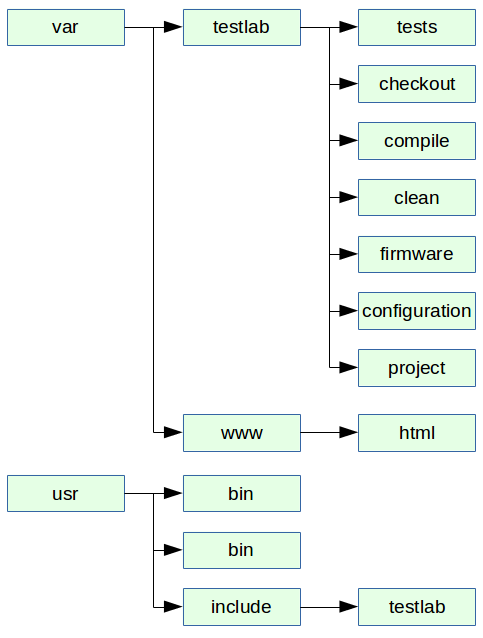
\includegraphics[width=.4\LW]{adresar_struktura}
  \caption{Adresářová struktura testovacího systému}
  \label{fig:adresar_struktura}
\end{figure}

Třetí část testovacího systému se nachází v adresáři /var/www/html. Tuto část testovacího systému tvoří samotné webové stránky testovacího systému

\section{Struktura databáze}
Jak již bylo dříve zmíněno všechny informace o testovaných zařízeních a výsldedcích testů jsou uloženy v databázi. K těmto účelům byla využita MySQL databáze. K databázi má přístup samotný testovací program testlab, všechny programy testovacího api a hlavně webová aplikace sloužící k adminitraci modelů testovaných zařízení a reportování výsledků testů. Pro organizované uchovávání všech dat byla navržena základní struktura databáze, která se časem s přibývající funkcionalitou testovacího zařízení může měnit. Jednotlivé tabulky této struktury jsou popsány v samostatných sekcích.

\subsection{Tabulka fwrelease}
První a základní tabulkou celého systému je fwreleases. V tabulce fwreleases jsou uloženy informace o testovaném releasu. Release je vytvořen a uložen do databáze při každém spuštění testování, aby bylo možné rozlišit různé testy. Všechny tabulky, které uchovávají informace o konkrétním testu odkazují právě na tuto tabulku. Tabulka fwreleases obsahuje pouze 3 údaje. Položka idfwreleases je primárním klíčem tabulky, položka date uchovává datum a čas vzniknu releasu a položka type určije o jaký typ vydání firmwaru se jedná.

\begin{figure}[h]
  \centering
  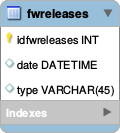
\includegraphics[scale=0.8]{database_fwreleases}
  \caption{Tabulka fwreleases}
  \label{fig:database_fwreleases}
\end{figure}

\subsection{Tabulka platforms}
Tabulka platforms obsahuje informace o jednotlivých platformách. Platforma je skupina výrobků postavena na společných zdrojových kódech a na jednom procesoru. Platformy se dále dělí na výrobky. Tabulka obsahuje prozatím následující 4 položky. Položka idplatforms, která je primárním klíčem tabulky, položka name slouží k uložení názvu tabulky, dále položky timeout\_checkout a timeout\_build sloužící k nastavení timeoutu skriptu pro stažení zdrojových kódu platfromy a pro přeložení zfrojových kódů platformy.

\begin{figure}[h]
  \centering
  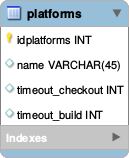
\includegraphics[scale=0.8]{database_platforms}
  \caption{Tabulka platforms}
  \label{fig:database_platforms}
\end{figure}

\subsection{Tabulka products}
Tabulka products obsahuje informace o jednotlivých produktech. V této tabulce nejsou produkty chápány jako jednotlivé produkty v testovací laboratoři, ale pouze jednotlivé druhy firmwaru. Rozdělení bylo provedeno z důvodu možnosti nahrání stejného firmwaru do různého hardwaru a tímto vznikne nový výrobek. Tabulka products obsahuje pouze 3 následující položky. Položka idproducts, které je primárním klíčem tabulky, položka idplatforms odkazující na danou platformu v tabulce platforms. Poslední položka name definuje název produktu.

\begin{figure}[h]
  \centering
  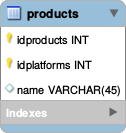
\includegraphics[scale=0.8]{database_products}
  \caption{Tabulka products}
  \label{fig:database_products}
\end{figure}

\subsection{Tabulka checkout}
Tabulka checkout slouží pro ukládání výsledků ze stažení zdrojových kódů z repozitáře. Tabulka obsahuje 4 položky. Položka idcheckout je primárním klíčem tabulky. Položka idplatforms odkazuje na tabulku platforms a udává o jaké zdrojové kódy platformy se jedná. Položka idfwreleases odkazuje na tabulku fwreleases a udává k jakému testování výsledek odpovídá. Poslední položka state ukládá stav výsledku skriptu pro stažení aktuálních zdrojových kódů platformy.

\begin{figure}[h]
  \centering
  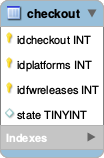
\includegraphics[scale=0.8]{database_checkout}
  \caption{Tabulka checkout}
  \label{fig:database_checkout}
\end{figure}

\subsection{Tabulka builds platform}
Tabulka builds\_platform slouží pro ukládání výsledků překladu celé platformy, čili všech výrobků dané platformy. Tabulka obsahuje celkem 4 položky. Položka idbuilds\_platform je primárním klíčem tabulky. Položka idplatforms odkazuje na tabulku platforms a udává jaké platformy se výsledek překladu týká. Položka idfwreleases odkazuje na tabulku fwreleases a udává k jakému vydání firmwaru je zdrojový kód překládán. Poslední položka state představuje stav ukončení překladu firmwaru pro celou platformu.

\begin{figure}[h]
  \centering
  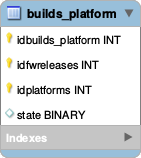
\includegraphics[scale=0.8]{database_buildsplatform}
  \caption{Tabulka builds platform}
  \label{fig:database_buildsplatform}
\end{figure}

\subsection{Tabulka build product}
Tabulka builds\_product slouží pro ukládání výsledků překladu jednotlivých výrobků. Tabulka obsahuje celkem 4 položky. Položka idbuilds\_product je primárním klíčem tabulky. Položka idproducts odkazuje na tabulku products a udává jakého produktu se výsledek překladu týká. Položka idfwreleases odkazuje na tabulku fwreleases a udává k jakému vydání firmwaru je zdrojový kód překládán. Poslední položka state představuje stav ukončení překladu firmwaru daného produktu.

\begin{figure}[h]
  \centering
  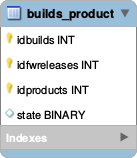
\includegraphics[scale=0.8]{database_buildsproduct}
  \caption{Tabulka builds product}
  \label{fig:database_buildsproduct}
\end{figure}

\subsection{Tabulka routers}
Tabulka routers je určena pro uložení všech routerů přítomných v testovací laboratoři. Položky v této tabulce tedy nepředstavují již dříve zmíněný produkt, ale skutečný výrobek. Každá položka této tabulky představuje model testovaného zařízení, tudíž testovány jsou pouze ty routery které jsou zde uloženy. Kompletní model zařízení netvoří pouze tato tabulka. Pro sestavení kompletního modelu jsou dále potřebné funkce a jejich přiřazení popsané v dalších tabulkách. Tabulka obsahuje tyto položky tvořící model zařízení. Položka idrouters je primárním klíčem tabulky. Položka idproducts odkazuje do tabulky products a definuje jaký firmware má být nahrán do tohoto výrobku. Položka idplatform odkazuje do tabulky platforms a definuje platformu na které je daný výrobek postaven. Další položka name slouží k pojmenování výrobku v testovací laboratoři, tato položka slouží pouze k snadnému rozeznání výrobků v testovací laboratoři. Položka port definuje v jakém portu switche je zapojen primární ethernet testovaného výrobku. Výchozí IP adresu tohoto primárního portu definuje položka address. Prozatím poslední položkou je protocol. Položka protocol určuje primární protocol pomocí kterého testovaný výrobek komunikuje s testovací aplikací.

\begin{figure}[h]
  \centering
  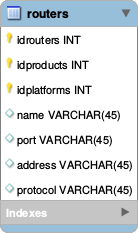
\includegraphics[scale=0.8]{database_routers}
  \caption{Tabulka routers}
  \label{fig:database_routers}
\end{figure}

\subsection{Tabulka functions}
Další tabulkou pomocí níž se tvoří model testovaného zařízení je tabulka functions. Tabulka functions sdružuje data o jednotlivých funkcích, které mohou testované výrobky podporovat. Tabulka obsahuje následující položky definující informace o dané funkci. Položka idfunctions je primárním klíčem tabulky. Položka name definuje název pod kterým je daná funkcionalita reprezentována všude v testovacím systému. Poslední položkou je položka order určující pořadí v jakém mají být funkcionality testovány.

\begin{figure}[h]
  \centering
  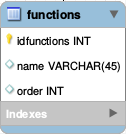
\includegraphics[scale=0.8]{database_functions}
  \caption{Tabulka functions}
  \label{fig:database_functions}
\end{figure}

\subsection{Tabulka dependences}
Třetí tabulkou tvořící model testovaného zařízení je tabulka dependences. Pomocí teto tabulky je možné definovat závisloti jednotlivých funkcí na jiných. Tudíž je možné definovat spuštění jednoho testu v závislosti na výsledku jednoho nebo více předešlých testů. Popsaná funkcionalita je realizována pomocí následujících třech položek. Položka target odkazuje na určitou funkci a určuje funkci, která je závislá na výsledku jiných funkcí. Položka dependences také odkazuje na určitou funkci a určuje na výsledku jaké funkce závisý provedění testů funkce target.
Poslední položka určuje typ závislosti. Podporovány jsou dva typy závislosti. Buď musí být správně otestovány všechny předešlé funkce nebo stačí úspěšný výsledek testů pouze jedné ze závislých funkcí.

\begin{figure}[h]
  \centering
  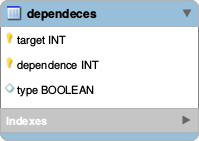
\includegraphics[scale=0.8]{database_dependences}
  \caption{Tabulka dependences}
  \label{fig:database_dependences}
\end{figure}

\subsection{Tabulka routers has functions}
Poslední tabulkou tvořící model testovaného zařízení je tabulka routers\_has\_functions. Pomocí této tabulky jsou každému modelu přiřazeny funkce, které je možné testovat. Přiřazení je realizováno pomocí dvou cizích klíčů odkazujících do tabulek routers a functions. Do tabulky routers odkazuje položka idrouters a položka idfunctions odkazuje do tabulky functions.

\begin{figure}[h]
  \centering
  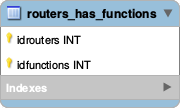
\includegraphics[scale=0.8]{databse_routershasfunctions}
  \caption{Tabulka routers has functions}
  \label{fig:databse_routershasfunctions}
\end{figure}

\subsection{Tabulka procedures}
Tabulka procedures již neslouží k uchování dat z abstraktního pohledu testování založeného na modelech. Tabulka uchovává jednotlivé spustitelné procedury sloužící k testování jednotlivých funkcí. Procedury jsou definované následujícímy položkami. Položka idprocedures je primárním klíčem tabulky. Položka idfunctions odkazuje na záznam v tabulce functions a definuje funkci kterou má procedura testovat. Položka name definuje název procedury pod kterým se spustitelný skript v testovacím systému reprezentuje. Položka unit slouží k lepší reprezentaci výsledku daného skriptu. Pokud procedura vrací hodnotu která je definována jakoukoliv jednotkou, může být zde tato jednotka definována. Položka timeout určuje čas maximálního běhu testovací procedury. Po uplynutí tohoto času je testovací procedura neúspěšně ukončena.

\begin{figure}[h]
  \centering
  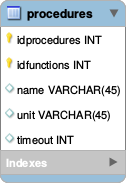
\includegraphics[scale=0.8]{database_procedures}
  \caption{Tabulka procedures}
  \label{fig:database_procedures}
\end{figure}

\subsection{Tabulka tests router}
Výsledky testování jsou ukládány do tří různých tabulek pro jednodušší reportování výsledků testování. První tabulkou je tests\_router do které jsou ukládány informace o testování celého produktu. Za úspěšný se tento test považuje pokud všechny procedury spustěné na testovaném zařízení zkončily úspěšně. Tabulka obsahuje 4 následující položky. Položka idtests\_router je primárním klíčem tabulky. Položka idrouters odkazuje na tabulku routers a určuje jakému zařízení je výsledek testu určen. Položka idfwreleases odkazuje na tabulku fwreleases a určuje k jakému vydání firmwaru je výsledek testu přiřazen. Poslední položkou je samotný výsledek testu a to položka result.

\begin{figure}[h]
  \centering
  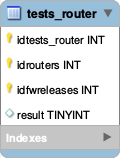
\includegraphics[scale=0.8]{database_testsrouter}
  \caption{Tabulka tests router}
  \label{fig:database_testsrouter}
\end{figure}

\subsection{Tabulka tests function}
Druhou tabulkou sloužící k ukládání výsledků testů je tabulka tests\_function. Tato tabulka sdružuje výsledky všech testovacíh procedur dané funkce na jednom testovaném zařízení. Test funkce je považován za úspěšný, pokud všechny testoavné procedury této funkce proběhli úspěšně. Tabulka tests\_function obshauje pět následujících položek. Položka idtests\_function je primárním klíčem tabulky. Položka idfunctions odkazuje na tabulku functions a definuje o jakou testovanou funkci se jedná. Položka idfwreleases odkazuje na tabulku fwreleases a definuje k jakému testovanému firmwaru je výsledek testování funkce přiřazen. Položka idrouters odkazuje na tabulku routers a definuje jakému zařízení je výsledek testu přiřazen. Poslední položka result určuje samotný výsledek testu.

\begin{figure}[h]
  \centering
  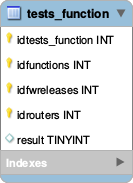
\includegraphics[scale=0.8]{database_testsfunction}
  \caption{Tabulka tests function}
  \label{fig:database_testsfunction}
\end{figure}

\subsection{Tabulka tests procedure}
Poslední tabulkou sloužící k ukládání výsledků testů je tabulka tests\_procedures.V této tabulce jsou uloženy vyýsledky ze všech spuštěných testovacích procedur. K identifikaci výsledku testu z každé testovací procedury slouží šest následujících položek. 
idtests\_procedure
idprocedures
idrouters
idfwreleses
result
value

\begin{figure}[h]
  \centering
  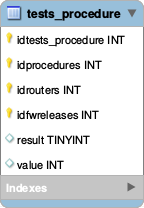
\includegraphics[scale=0.8]{database_testsprocedure}
  \caption{Tabulka tests procedure}
  \label{fig:database_testsprocedure}
\end{figure}

\subsection{Tabulka logs}
Tabulka logs schromažďuje všechny chybové výpisy vygenerovány testovacímy skripty. Tabulka obsahuje pět následujících položek. Položka idlogs je primárním klíčemm tabulky. Položka idprocedures odkazje na tabulku procedures a definuje jaké testovací procedury se chybová hláška týká. Položka idrouters odkazuje na tabulku routers a definuje jakého testovaného zařízení se chybová hláška týká. Položka idfwreleases odkazuje na tabulka fwreleases a definuje jakého firmwaru se chybová hláška týká. Poslední položka event určuje samotný text chybové hlášky.

\begin{figure}[h]
  \centering
  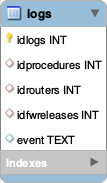
\includegraphics[scale=0.8]{database_logs}
  \caption{Tabulka logs}
  \label{fig:database_logs}
\end{figure}

\section{Popis programu}

O průběh celého testu se stará program testlab. Testlab je program psaný v jazyc C. Program po spuštění otevře systémový log pro možnost logování chyb do systémového logu. Filtrováný systémový log by měl později být zobrazován na webowém rozhraní testovacího systému. První hláškou do systémového logu je informace o spuštění programu testlab, daným uživatelem a v určený čas. Po otevření systémového logu program rozebírá parametry na příkazové řádce. Parametry jsou rozebíráný pomocí funkce getopts. Pomocí parametrů lze ovlivnit chování programu testlab !!!!!DOPLNIT PARAMETRY!!!!!!

\begin{figure}[h]
  \centering
  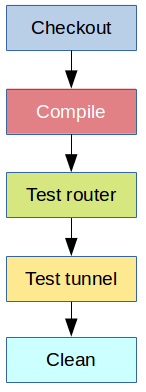
\includegraphics[width=.2\LW]{program_schema}
  \caption{Základní schéma testovacího programu}
  \label{fig:program_schema}
\end{figure}


Nyní se provádějí přípravné kroky pro samotné testování. Nejdříve je vytvořen nový release firmwaru a následně vložen do databáze. V projektovém adresáři je vytvořen nový adresář se stejným názvem jako identifikační číslo testovaného releasu.

\subsection{Checkout}
\subsection{Compile}
\subsection{Test router}
\subsection{Test tunel}
\subsection{Clean}
\subsection{Remote server}
\subsubsection{Telnet}
\subsubsection{SSH}

\endinput

  \chapter{API pro psaná testů}


\endinput

  \chapter{Uživatelský interface}


\endinput

  \chapter{Návrh testů pro Conel routery}
V této fázi je připraven celý systém pro testování routerů. Testovací laboratoř se všemi výrobky je kompletně postavena. Testovací server je nainstalován a nakonfigurován. Máme navrhnutou databázi a adresářovou strukturu tetovacího systému. Systém pro stahování zdrojový kódů, kompilování projektů a následné spouštění testů již také funguje správně. Pro provádění jednotlivých kroků testů jsou k dispozici programy z testovacího API a výsledky všech testů je možné zobrazit pomocí webového interfacu.

V neposlední řadě je navrhnut přístup testování založený na modelech. Pomocí tohoto přístupu rozdělíme všechny funkcionality všech routerů do funkcí. Následně každou funkci rozdělme na jednotlivé procedury, kdy každá procedura testuje elementární chování této funkce. Například pokud je dána funkce připojení routeru do mobilní sítě a v této funkci je testovací procedura testující změny APN tohoto připojení. Pomocí těchto funkcí je možné možné namodelovat všechny routery. Pomocí těchto modelů jsou pro každý router vybírány a spouštěny konkrétní testy.

Pro základní testování funkčnosti celého portfolia výrobků společnosti Conel byli navržený následující funkce a testovací procedury. V první fázi implementace testovacího systému budou spouštěny tyto níže popisované procedury.

Testovací skripty jsou spouštěny se dvěma parametry. Prvním parametre je identifikační číslo testovaného zařízení. Pomocí tohoto čísla je možné komunikovat s daným zařízením a zjišťovat detailní informace o zařízení z databáze pomocí programů posaných v sekci věnující se testovacímu API. Druhým parametrem je předáváno identifikační číslo testovaného releasu.

\section{Checkout}
Testování každého projektu je započato stažením zdrojových kódů daného projektu. Způsob stažení zdrojového kódu je zajištěno pomocí skriptů checkout. V tomoto skriptu definujeme způsob stažení zdrojový kódu. Například stažení pomocí verzovacích systémů git, či cvs nebo zkopírování projektu z určiého místa. Všechny projekty testovacího systému se stahují pomocí verzovacího systému git přímo ze serveru testovací laboratoře, kde jsou vytvořeny kopie repozitářů všech testovaných projektů. Kopie je pravidelně každou minutu udržována aktuální. Tento postup byl zaveden z důvodu zrychlení samotného testování a rapidní zmenšení datových toků. Primárně je stahována hlavní větev master.

\section{Compile}
Pro každý projekt je dále napsán skript zajišťující kompilaci daného projektu a vybraného produktu. Skript je pouště se dvěma parametry. Prvním parametrem je cílový adresář kam má být výsledný firmware nakopírován a druhým parametrem je název překládaného výrobku. Prozatím se pro všechny testované projekty používá buildovací systém ltib, tudíž skipty zajišťující překlad projektů vypadají velice obdobně. Každý skript je prováděn v adresáři kde je projekt stažen. V prvním kroku je otevřen adresář ltib. Dále pokud se překládá první výrobek platformy, tak je vybrána zpracovávaná platforma. Samotné vybrání platformy je provedeno ve dvou krocích. V prvním kroku je spuštěn skript platform s parametrem název platformy. Skript platform byl do buildovacího systému doplněn v rámci testovací laboratoře, jelikož ltib nepodporoval překládání bez interakce uživatele. Výběr platformy je dokončen spuštěním programu ltib v konfiguračním režimu. V dalším kroku je vybrán produkt, který má být překládán. Vybrání produktu je provedeno zapsáním jeho názvu do soubouru appname. Nyní jsou smazány přeložené části závisející na výrobku a spuštěn samotný překlad. V případě úspěšného ukončení překladu jsou přeložené firmwary nakopírovány do adresáře předaného jako paramter skriptu. Překládání projektů pomocí skriptů bylo zvoleno z důvodu univerzálnosti a jednoduchém přidávání nových projektů založených na různých buildovacích systémech.

\section{Clean}
Před ukončením testování je prováděn úklid po kompilaci projektů. Aby bylo možné smazat všechny soubory a adresáře zdrojových kódu a soubory vytvořené při samotoném překladu je nutné provést clean nad projektem. Jelikož clean každého projektu je prováděn odlišným způsobem  je pro každý projekt vytvořen vlastní skript. Pro projekty, které jsou zatím testovány v testovací laboratoři je nejdří otevře adresář ltib. Samotný úklid po překladu je provededen spuštěním programu ltib v módu distclean. Na závěr se skript vrátí do výchozího adresáře a je ukončen s návratovým kódem programu ltib.

\section{Funkce firmware}
Základní funkcionalitou každého výrobku je možnost nahrání nového firmwaru. Na funkci nahrání nového firmwaru je založeno všechno další testování. Pokud se nepodaří nahrát nový firmare není důvod testovat jakoukoliv funkcionalitu, jelikož tyto testy neodpovídají danému firmwaru.

\subsection{Procedura upload}
První testovací procedura funkce firmware testuje nahrání firmwaru do testovaného zaříení. V prvním kroku je zjištěn název firmwaru testovaného zařízení z databáze testovacího systému. Dále je správný firmware nahrán do testovaného zařízení pomocí utility updatefw z testovacího API. Test je ukončen úspěšně pokud se podaří nahrát firmware do zařízen.

\subsection{Procedura start}
Dalši testovací procedura funkce firmware testuje jestli router po nahrání firmwaru nastartoval. V tomto testu se nejdříve jednu sekundu čeká na reboot routeru po ukončení programování, jelikož pokud by se router testoval ihned po naládování testoval by se ještě běžící starý firmware. Dále je spuštěn program testující připojení routeru do testovací sítě. V tomto programu je nejdříve testován ping na router a v případě úspěšného pingu je testováno odezva routeru na příkaz echo. Test končí úspěšně pokud se na routeru podaří ping a také se k němu podaří připojit jedním z podporovaných protokolů. Tento test vrací také čas v sekundách za jak dlouho trval start routeru.

\subsection{Procedura check}
Poslední procedura funkce firmware check testuje shodu verzi firmwaru v routeru s nahrávanou verzí verzí firmwaru testovacím systémem. V první fázi je z databáze zjištěn název firmwaru testovaného výrobku. Pomocí názvu firmwaru je nalezen a jeho obsah uložen do proměné soubor s verzí firmwaru dodávaný s přeloženým firmware. Po zjištění požadovaného firmwaru je zjištěn aktuální firmware v routeru pomocí programu status. Nakonec jsou tyto dvě verze porovnány a skript je úspěšně ukončen pokud jsou obě verze totožné.

\section{Funkce configuration}
Další funkcionalitou, kterou podporují všechny testované zařízení je funkcionalita obsluhující konfigurace. Konfigrace zařízení je seznam parametrů s hodnotami určující chování daného zařízení. Tato funkcionalita je také velmi důležita, jelikož v každém testu je nastavována odlišná konfigurace a sleduje se chování daného zařízení. Pro práci s konfigurací je v routerech několik základních nástrojů. Konfigurace je možné zálohovat a nahrávat nové. Dále je možné pracovat s takzvanými profily. K dispozici jsou až řtyři alternativní profily. Nakonec je možné měnit parametry přímo v routeru přepisováním určitých souborů.

\section{Funkce connect}
Nyní přicházejí dvě základní funkcionality, které obstarávají připojení do routeru. K dispozici jsou dvě možnosti připojení do testovaných zařízení. Ne všechny testovaná zařízení podporují oba typy připojení. První typ připojení do routeru je pomocí klasických nešifrovaných protokolů telnet, ftp, http. Jedná se o nezabezpečené připojení, tudíž není podporováno nejnovějšími zařízení platformy v3.

\subsection{Procedura telnet}
První procedura telnet testuje připojení do routeru pomocí protokolu telnet. Nejdříve je zjiště původní komunikační protokol, aby bylo možné před ukončením testu protokol zpět obnovit. Komunikační protokol je zjištěn z remote serveru pomocí programu remoteinfo z testovacího API. Dále je remote serveru odeslán požadavek na změnu komunikačního protokolu pomocí programu remotechange. Po změně protokolu je kontrolováno jestli se protokol opravdu změnil a to opět pomocí programu remoteinfo. Na závěr je provedena zkouška komunikace pomocí telnet protokolu. Zkouška komunikace je provedena pomocí programu remote a příkazu echo, následná kontrola komunikace je prováděna porovnáním vráceného řetězce s řetězcem vypisovaným příkazem echo. Posledním krokem tohoto testu je vrácení původního komunikačního protokolu remote serveru.

\section{Funkce connect ssh}
Druhým možným způsobem komunikace s testovanými zařízeními je pomocí zabezpečeného šifrovaného protokolu ssh. S podporou protokolu ssh souvisejí i další šifrované typy připojení klasických protokolů. Například zabezpečená varianta ftps protokolu pro přenos dat ftp, dále šifrovaná varianta https webové protokolu http. Zabezpečené šifrované protokoly nepodorují kvůli malému výkonu starší modely testovaných zařízení, naopak nejnovější modely zařízení podporují pouze tento druh spojení.

\subsection{Procedura ssh}
Procedura ssh testuje spojení s testovaným zařízením skrz šifrovaný protokol ssh. Připojení protokolem ssh je prováděno pomocí programu plink, jelikož standardní ssh klient nedovoluje zadání hesla připojení jako parametr. Tato funkcionalita je stejně jako telnet zaintegrována do remote serveru, tudíž je možné se k ssh spojení chovat stejně jako k telnet spojení. Díky tomuto faktu vypadá testovací procedura totožně jako testovací procedura pro telnet s jediným rozdílem. Při změně protokolu pomocí programu remotechange se jako parametr nepředává telnet nýbrž řetězec ssh. Podmínka úspěšnosti provedení testu je taktéž totožná s procedurou telnet.

\section{Funkce mobile}
Nyní již jsou popsány všechny funkcionality nutné k testování všech zařízeních a přejdeme k popisu všech ostatních funkcionalit. První testovaná funkcionalita je funkce mobile. Funkce mobile v sobě obsahuje společný základ všech bezdrátových možností připojení. Základními vlastnostmi připojení jsou například přiřazení IP adresy, zkouška komunikace či změna parametru určující velikost odchozího packetu MTU. Jednotlivé vlastnosti této funkcionality jsou popsány v testovacích procedurách testujících tuto vlastnost.Tato funkce naopak nezohledňuje typ spojení bezdrátového modulu s routerem, či podporované bezdrátové technologie.

\subsection{Procedura connect}
Procedura connect popisuje vlastnost routeru připojení pomocí mobilního spojení. Úspěšné připojení do mobilní sítě je definováno přiřazením IP adresy interfacu mobilního spojení. Samotný test probíhá pouze spuštěním programu mobileready, který čeká 3 minuty na přiřazení IP adresy interfacu mobilního spojení. Program, tedy i skript vypisuje pouze čas v sekundách, který čekal na připojení routeru do mobilní sítě. Skript je ukončen úspěšně pokud se routeru podaří připojit do mobilní sítě do třech minut.

\subsection{Procedura ping}
Procedura ping popisuje vlastnost routeru základní komunikace v mobilní síti. Vlastnost základní komunikace je popsána provedením provedením alespoň jednoho úspěšného pingu na zařízení v mobilní síti. Samotný test probíhá následovně. V prvním kroku je zálohováno původní APN. Poté je změněno APN mobilního spojení na conel.agnep.cz, aby byla na všemi routery přístupná jedna stejná adresa. Kvůli projevení změny APN je proveden restart služby PPP starající se o mobilní spojení. Po restartu mobilního spojení je čekáno na sestavení mobilního spojení s novým APN pomocí programu mobileready. V případě úspěšného návázání mobilního spojení je proveden ping s pěti pokusy na adresu 10.0.0.1. Na závěr je parametru APN navrácená původní hodnota. Skript vypisuje číselnou hodnotu v procentech počtu úspěšně provedených pingů. Test je ukončen jako úspěšný jestliže byl úspěšně přijat zpět alespoň jeden pokus o ping na adresu 10.0.0.1.

\subsection{Procedura apn}
Procedura apn popisuje možnost ovlivnění chování mobilního spojení pomocí parametru APN. Parametr APN určuje síť ke které se testované zařízení připojuje. Testovaná zařízení typicky obsahují SIM karty podporující firemní apn conel.agnep.cz a APN umožňující přístup do internetu internet.t-mobile.cz. Test vlastnosti zkoumá jestliže se změní síť mobilního připojení při změně parametru APN. Samotný test probíhá následovně. Nejdříve je zálohováno původní APN. Následuje změna APN na conel.agnep.cz. Kvůli projevení změny APN je proveden restart mobilního spojení. Dále pomocí programu mobileready je čekáno na sestavení mobilního spojení. Po sestavení mobilního spojení je zjištěna přidělená IP adresa mobilního interfacu. Stejný postup je proveden pro zadání prázdného APN. V případě pokud se router v obou zadaných APN připojil do mobilní sítě jsou porovnávány IP adresy připojení v obouch případech. Jestliže jsou IP adresy různé , tak je funkcionalita správná a test ukončen úspěšně.

\subsection{Procedura address}
Procedura address popisuje vlastnost mobilního spojení přiřazující IP adresu rozhraní mobilního spojení. Pokud známe IP adresu SIM karty v určitém APN můžeme zadat tuto adresu jako parametr mobilního spojení. Při vytváření mobilního spojení se použije tato adresa a vytvoření spojení by se mělo provést rychleji. Test této funkcionality odpovídá zadáním IP adresy SIM karty a úspěšném vytvoření spojení. Test je prakticky implementován následovně. Nejdříve je zálohovány parametry routeru IP adresa a APN. Poté je z databáze zjištěna IP adresa SIM karty vložené do testovaného routeru. Po zjištění IP adresy je tato adresa zadána jako parametr mobilního spojení, druhým měněným parametrem je APN pro které je tato adresa použita. Pro kontrolu funkčnosti zadání IP adresy je restartováno mobilní spojení a pomocí programu mobileready je čekáno na sestavení mobilního spojení. Skript je úspěšně ukončen jestliže IP adresa SIM karty získaná z databáze je totožná s IP adresou SIM karty přidělené mobilnímu rozhraní. Skript nadále vypisuje čas v sekundách za jak dlouho se router připojil do mobilní sítě. Na závěr skript navrátí původní nastavení routeru.

\subsection{Procedura operator}
Procedura operator popisuje vlastnost určení operátora mobilního spojení. Operátor je určen pětimístným číselným kódem. Zadáním parametru operátor je urychleno připojení do mobilní sítě, či změnit operátora, pokud to SIM karta umožňuje. Testování této vlastnosti mobilního spojení probíhá následovně. V první fázi je zálohována nynější položka konfigurace operátor. Poté je z databáze zjištěn operátor SIM karty testovaného zařízení. Získaný operátor je zadán jako nový parametr testovaného zařízení operátor. Z důvodu provedení změny v konfiguraci je proveden restart mobilního spojení a dále je čekáno na znovu sestavení mobilního spojení. Pokud bylo spojení úspěšně navázáno je porovnáván přidělený operátor s operátorem zadaném jako parametr, jestliže jsou tyto operátoři totožné je skript ukončen s nulovým návratovým kódem. Skript tiskne na standardní výstup dobu sestavování spojení se zadaným operátorem v konfiguraci.

\subsection{Procedura mtu}
Procedura mtu popisuje vlastnost mobilního spojení ovlivňující velikost odesílaného packetu. Při změně tohoto parametru bychom měli sledovat změnu velikosti odesílaných packetů. Testování změny parametru MTU je prováděno následujícím způsobem. Nejdříve je zálována nynější hodnota MTU a nastavíme novou hodnotu MTU na 500. Pro aplikaci změn v nastavení necháme restartovat mobilní spojení a počkáme na znovu navázání tohoto spojení. Po připojení testovaného zařízení do mobilní sítě je zjištěn název rozhraní mobilního spojení pro účely diagnostiky provozu sítě. Dále je v routeru na pozadí spuštěn ping s velikostí větší než nastavená maximální velikost packetu. Ping na pozadí je spouštěn pomocí programu z testovacího API pingb. V průběhu pingu je v testovaném routeru zároveň puštěn program pro monitorování sítě tcpdump. Pomoc9 tcpdumpu je po dobu 3 sekund sledovány odchozí packety typu icmp request na mobilním rozhraní. Po příchodu logu z tcpdumpu je kontrolována velikost odesílaných packetů. Jestliže velikost některých packetů je rovna maximální velikosti packetů je test úkončen s nulovým návratovým kódem, tedy byl ukončen úspěšně.

\section{Funkce mobile edge}
Funkcionalita mobile edge popisuje možnost připojení testovaného zařízení do mobilní sítě skrz techologie GPRS a EDGE. Tyto technologie nepodporují všechny zařízení, která mají vlastnost mobilního připojení, z toho důvodu byla pro tuto vlastnost vytvořena samostatná funkcionalita. Testované zařízení se k technologii edge připojují jestliže v místě použití není dostupná lepší technologie, či zařízení lepší technologii nepodporuje nebo je možné správným parametrem vynutit připojení routeru do mobilní sítě skrze tuto technologii.

\subsection{Procedura type edge}
Procedura type edge popisuje možnost připojení zařízení do mobilní sítě skrz technologii EDGE. Možnost připojení technologií edge je testována vynucením technologie EDGE a čekáním na navázání spojení pomocí teto technologie. Test testující tuto vlastnost probíhá následovně. V prvním kroku je zálohován původní typ sítě pro pozdější obnovení a nastavíme nový typ sítě na typ GPRS/EDGE. Z důvodu projevení nastavených změn je restartováno mobilní spojení a dále je čekáno na nové sestavení spojení. Po úspěšném sestavení spojení je pomocí programu status zjištěna technologi pomocí které je testované zařízení připojeno do mobilní sítě. Test je ukončen úspěšně pokud zjištěný typ sítě odpovídá nastavené technologii EDGE. Na závěr testu se pouze nastaví zpět původní typ technologie.

\section{Funkce mobile umts}
Funkcionalita mobile umts popisuje vlastnost připojení zařízení do mobilní sítě pomocí technologie UMTS a HSPA. Tyto technologie nepodporují všechny zařízení umožňující mobilní spojení. Například CDMA routery nepodporují GPRS přenosy, EDGE routery podporují maximálně technologie typu EDGE. Naopak LTE routery podporují i nižší technologie UMTS a EDGE. Zařízení komunikuje technologií UMTS jestliže nepodporuje nebo v místě použití není k dispozici lepší technologie nebo jesliže je správným parametrem vynucena technologie UMTS.

\subsection{Procedura type umts}
Procedura type umts popisuje možnost připijení zařízení do mobilní sítě skrz technologii UMTS. Testování technologie UMTS je prováděna totožným způsobem jako testování předešlé technologie EDGE. Jediným rozdílem v smatoném testu je že místo technologie EDGE se nastavuje technologie UMTS a zjištěná technologie je porovnávána s technologií UMTS.

\section{Funkce mobile lte}
Funkcionalita mobile lte popisuje vlastnost připojení zařízení do mobilní sítě pomocí technologie LTE. Technologie LTE je v nynější době nejrychleší a nejvyspělejší bezdrátovou technologií podporovanou zařízeními společnosti Conel. Možnost komunikovat pomocí technologie LTE mají pouze LTE routery. Naopak tyto routery mají možnost komunikovat mimo LTE technologie i pomocí EDGE a UMTS technologií.

\subsection{Procedura type lte}
Procedura typu lte popisuje možnost připojení zařízení do mobilní sítě skrz technologii LTE. Testování technologie LTE je proáděno totožným způsobem jakou u předešlých technologiíí EDGE a UMTS. Jedniým rozdílem v testovací proceduře je nastavování technologie LTE v konfiguraci a porovnávání vyčtené technologie s technologií LTE.

\section{Funkce mobile ppp}
Funkcionalita mobile ppp popisuje připojení zařízení do mobilního spojení pomocí protokolu ppp. Protokol ppp neboli point to point protokol je standardní protokol linkové vrsty používaná v telekomunikaci. Chování testovaných zařízeních komunikujících tímto protokolem můžeme změnit například změnou autentizace, či vytáčeného čísla. Protokol ppp používají vesměs zařízení se staršímy modely bezdrátových modulů, jelikož se jedná o velmi starý protokol, který je v dnešní době nahrazován novějšími a rychlejšími protokoly.

\subsection{Procedura chap}
Procedura chap popisuje vlastnost připojení protokolem ppp pomocí autentizace chap. Ve výchozím stavu router vybírá jednu z autentizací pap či chap a pomocí té se přihlásí do mobilní sítě. Výchozí chování lze ovlivni změnou parametru autentizace na autentizaci chap, poté se bude router přihlašovat do sítě jedině autentizací chap. Testování zvolení autentizace chap probíhá následujícím způsobem. Nejdříve je zálohován původní typ autentizace a autentizace je nastavena na chap. Pro projevení změny typu atentizace je potřeba restart ppp spojení. Dále je čekáno na nové sestavení spojení se zvolenou atentizací. Po sestavení spojení je v logu hledána hláška od deamona pppd hlásící úspěšné přihlášení do sítě pomocí autentizace chap. Test končí úspěšně jestliže je hláška "CHAP authentication succeeded" nalezena, v opačném případě skript končí s chybovým návratovým kódem.

\subsection{Procedura pap}
Procedura pap popisuje vlastnost připojení routeru do mobilní sítě protokolem ppp pomocí autentizace pap. Chování a nastavování autentizace již bylo popsáno v proceduře věnující se autentizaci chap. Samotné testování této autentizace je také shodné s testováním autentizace chap, až na dvě drobné změny. Při nastavování autentizace je nastavena autentizace PAP a hledaná hláška logu je změněna na "PAP authentication succeeded".

\subsection{Procedura number}
Procedura number popisuje vlastnost ppp spojení určující vytáčené číslo tímto spojením. Defaultně je vytáčené číslo zajišťující správné spojení, avšak v oddůvodněěných případech můžeme toto číslo pomocí parametru number změnit. Změna čísla se projeví změnou čísla v at komandu atd. Test vlastnosti probíhá následovně. Nejdříve je zálohováno původní telefoní číslo a nastaveno jakékoliv jiné číslo. Z důvodu projevení změny vytáčeného čísla je restartováno mobilní spojení. Po restartu mobilního spojení je po dobu 30 sekund sledován systémový log testovaného zařízení a je vyhledávaný at komand atd s parametrem zadaného čísla v konfiguraci. Test je prohlášen za úspěšný jestliže je daný komand v logu nalezen. Nakonec je navráceno původní telefoní číslo a mobilní spojení je restartováno.


\endinput

  \chapter{Testovací laboratoř v praxi}

Nyní je všechna softwarová část testovací laboratoře připravena k použití a je potřeba vše začít testovat na fyzickém hardwaru. Pro osazení všech částí testovací laboratoře byl vytvořen speciální stojan. Stojan má ve spodní části poličky na různá vybavení. V poličkách je prozatím umístěn testovací server a konfigurovatelný switch. Horní část stojanu tvoří DIN lišty sloužící k umístění testovaných zařízení. Celkem je zde umístěno deset DIN lišt po dvou metrech. Pro jednodušší vedení kabeláže jsem na stojan připevnil plastové ranžírovací panely.

\begin{figure}[h]
  \centering
  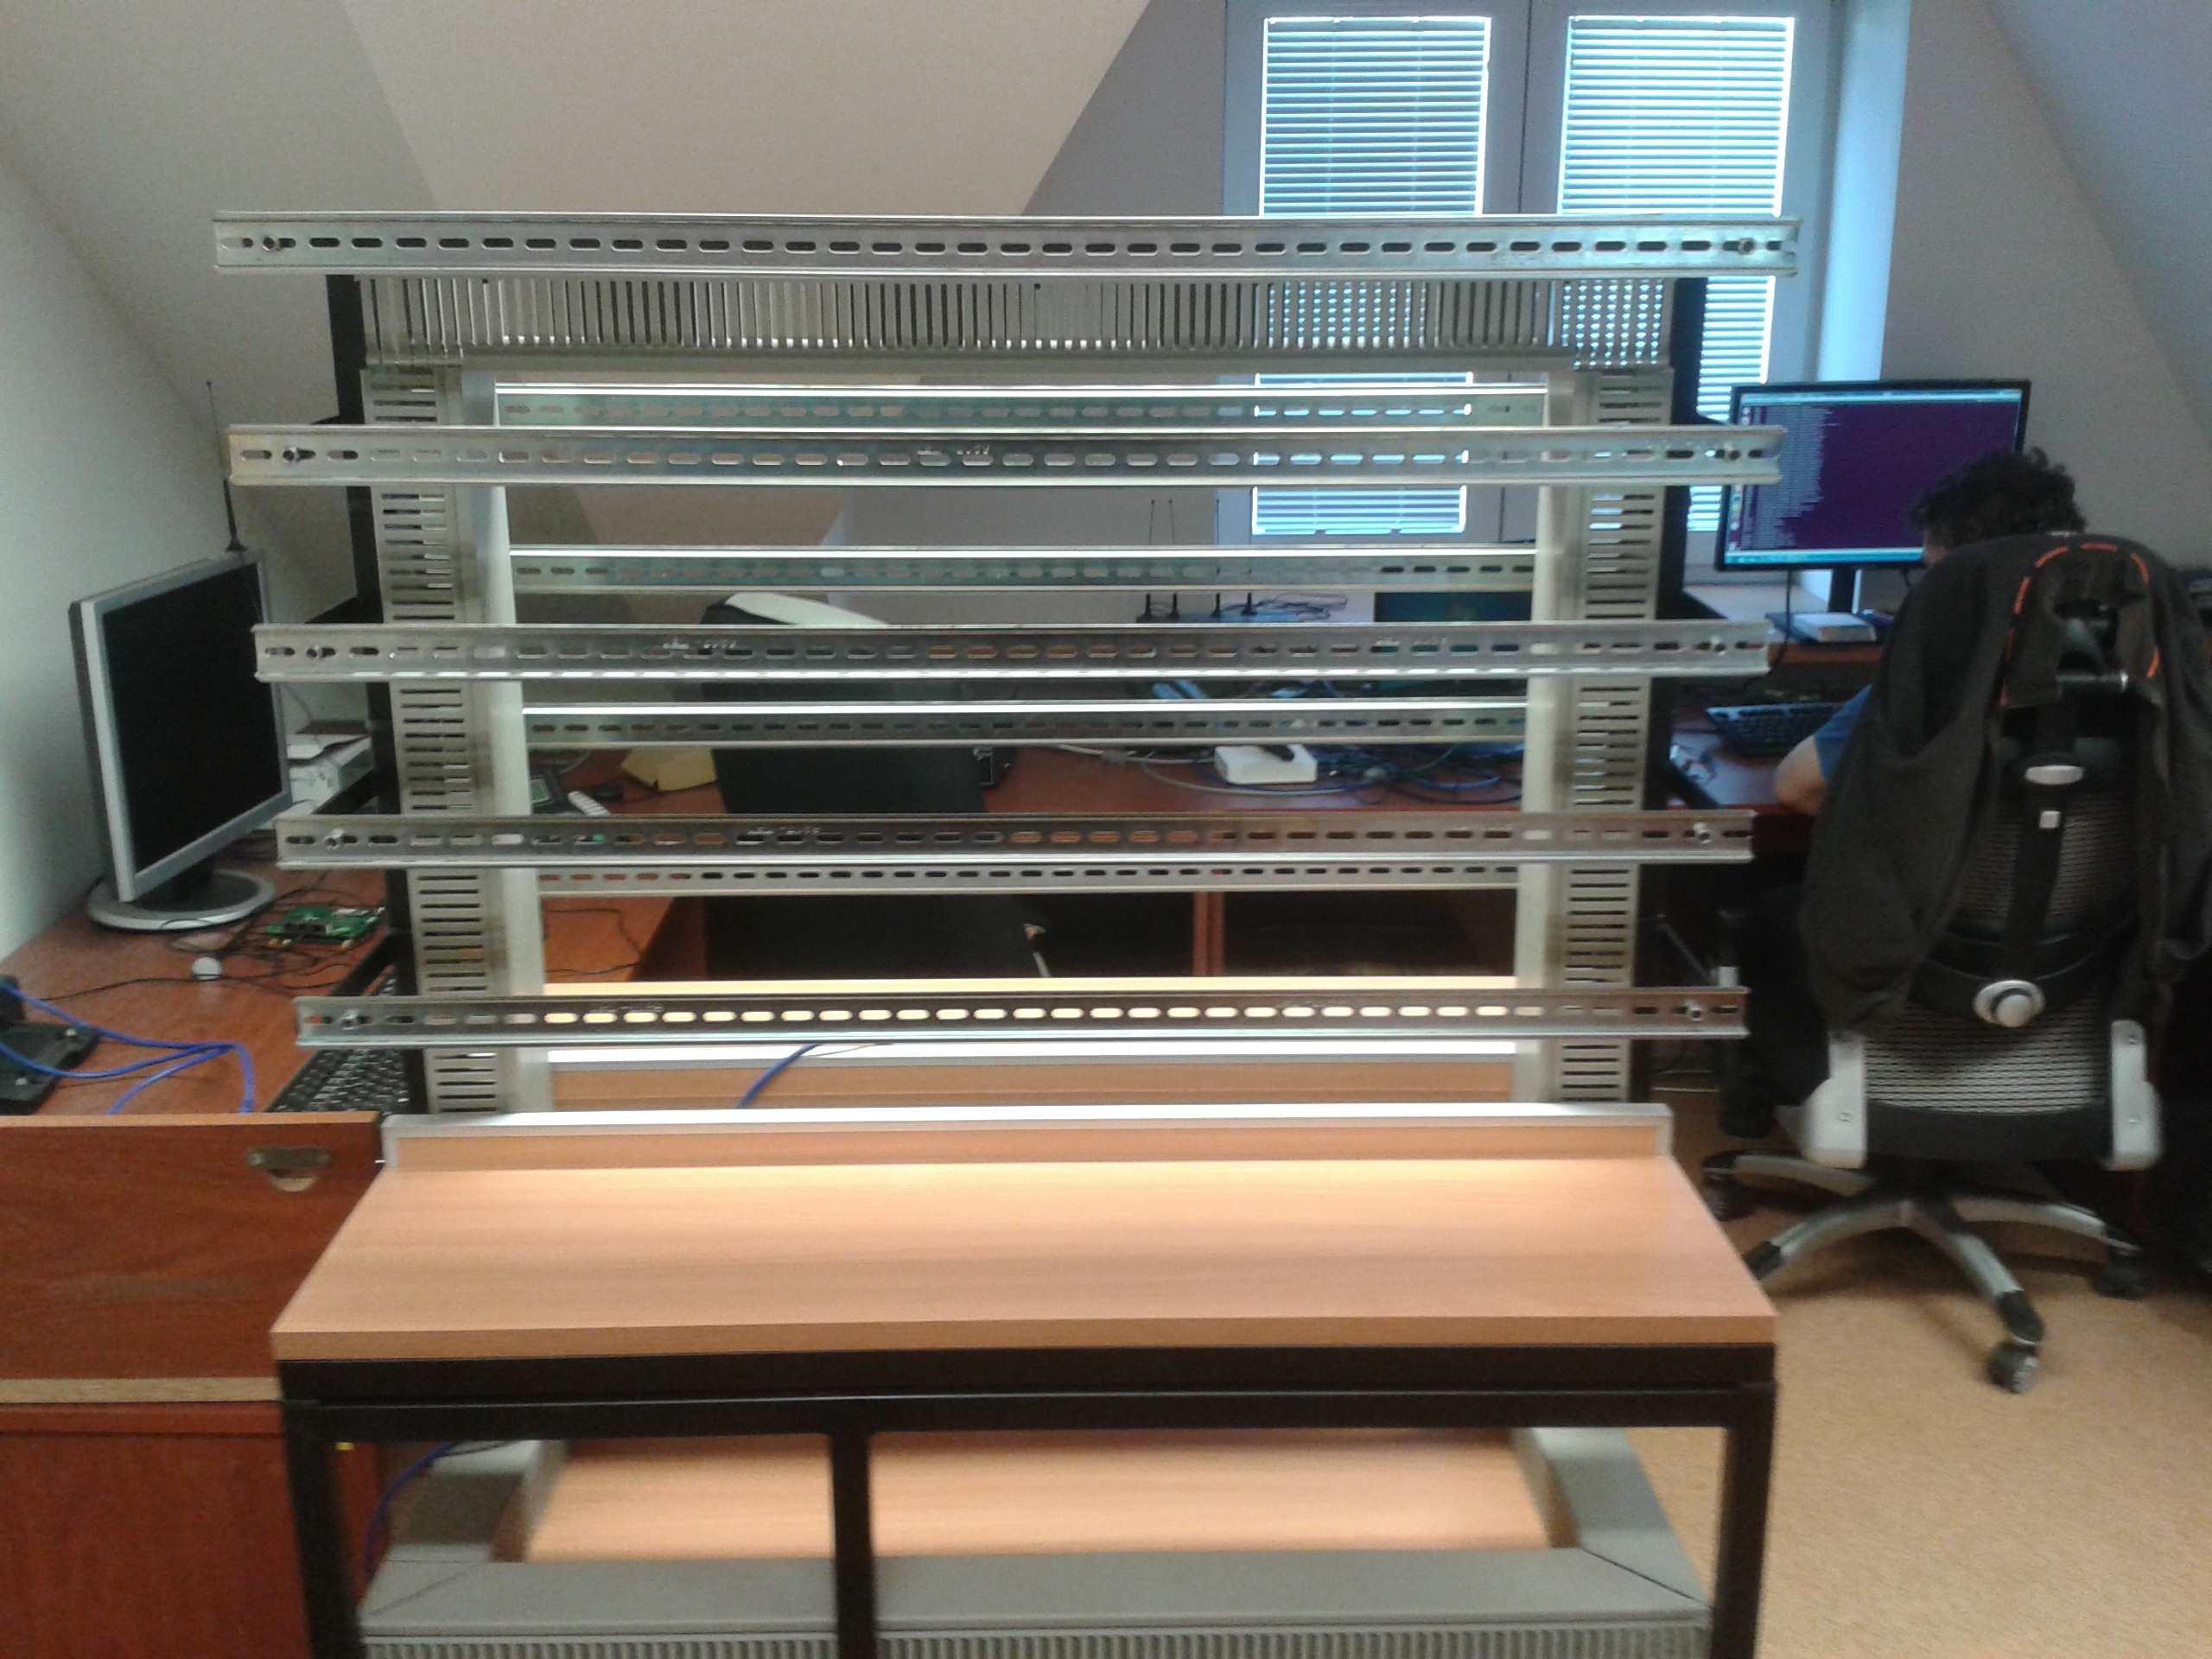
\includegraphics[width=\LW]{stojan1}
  \caption{Neosazený stojan}
  \label{fig:stojan1}
\end{figure}

Pro první fázi nasazení testování budu muset rozvést napájení a LAN síť. Napájení jsem řešil pomocí jednoho spínaného zdroje s možností montování na DIN lištu. Samotný zdroj má pouze dvě svorky na výstupní napájení, tudíž jsem vedle zdroje umístil svorkovnice na DIN lištu pro rozvedení napájení všech třiceti testovaných zařízení. Napájecí kabely  testovaných zařízení jsou dále vedeny ranžírovacím panelem a rovnoměrně po celé délce stojanu vyvedeny ven. Ethernetové kabely jsem vedl od switche umístěného ve střední polici stojanu do~svrchního ranžírovacího panelu, kde jsou Ethernetové kabely také rovnorměrně vyvedeny ven. Tímto rozložením jsem vytvořil univerzální stojan, kde pro připojení nového zařízení stačí pouze zařízení připevnit na DIN lištu, připojit napájení a Ethernet pomocí volně visících kabelů.

\begin{figure}[h]
  \centering
  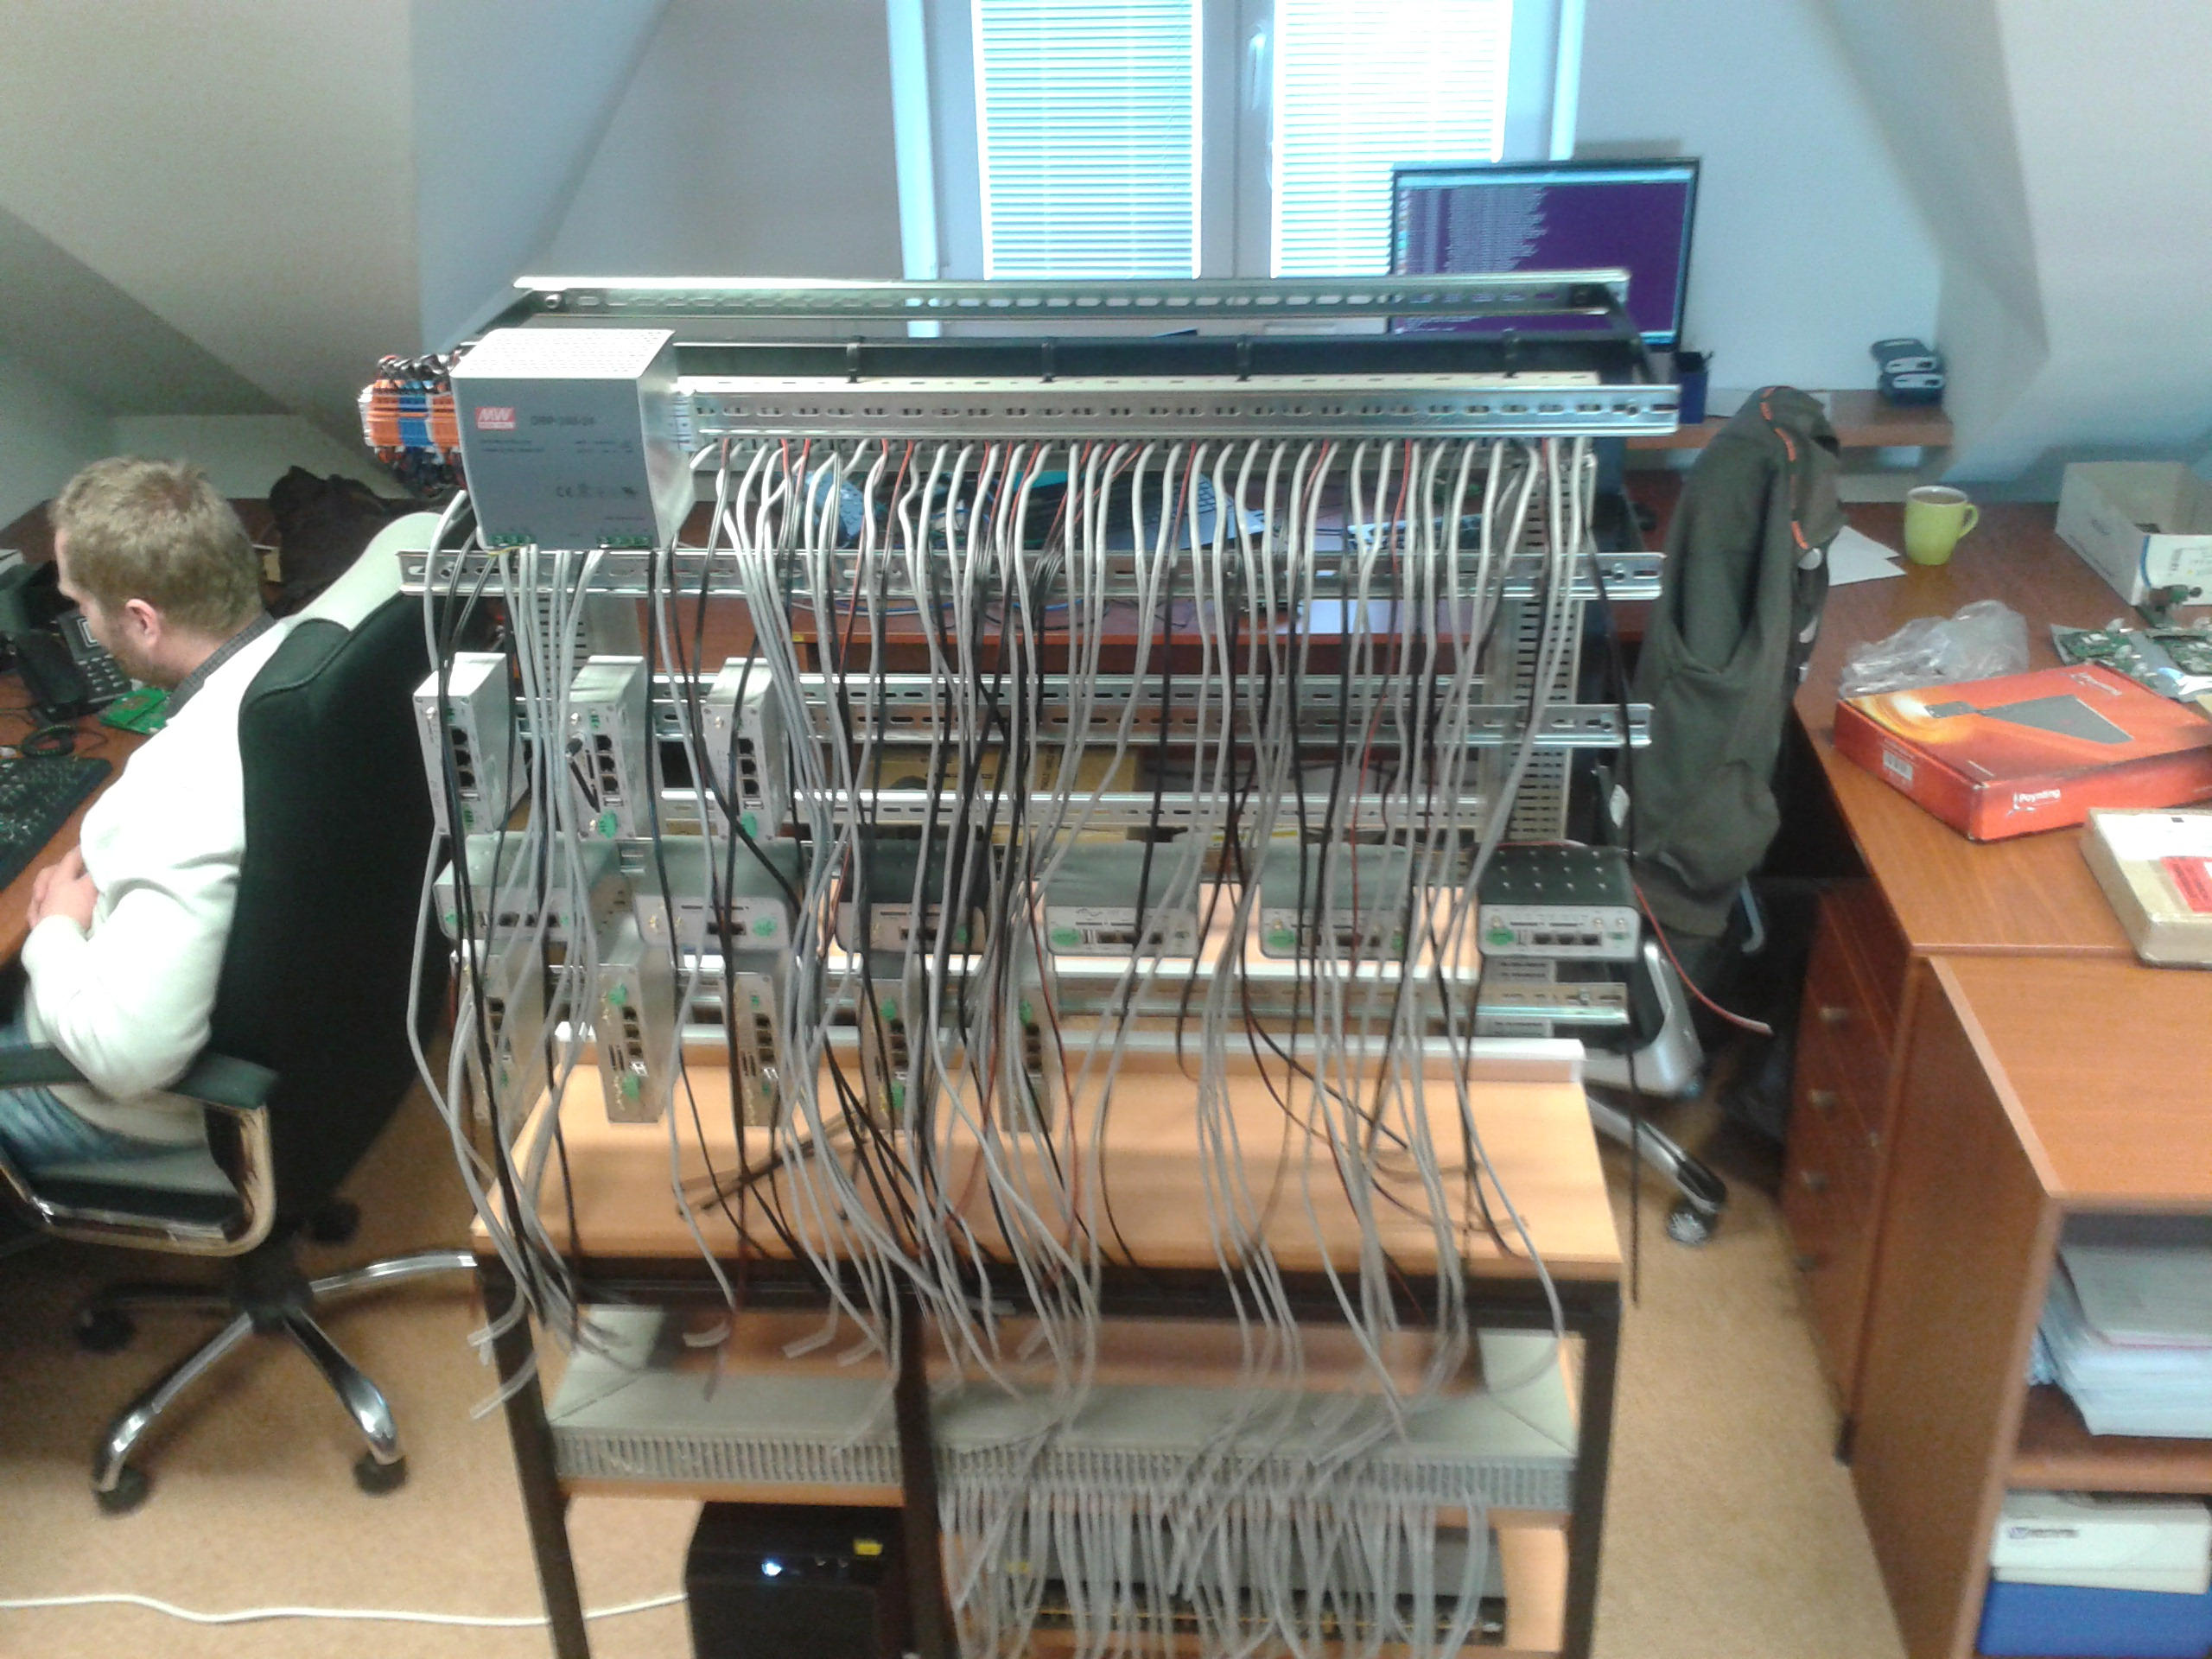
\includegraphics[width=\LW]{stojan2}
  \caption{Příprava kabeláže na stojan}
  \label{fig:stojan2}
\end{figure}

Posledním krokem potřebným pro uvedení testovací laboratoře do~provozu je připojení všech testovaných zařízení. Do~testovací laboratoře jsem zapojil všechny dostupné routery společnosti Conel.

Po zapojení všech testovaných výrobků jsem testovací laboratoř spustil a zahájil testovací provoz, kdy je každý den proveden překlad a test všech výrobků. Při pravidelném testování jsem prozatím nenašel závažné nedostatky. Občasné nepřipojení zařízení do~mobilní sítě je způsobeno velmi slabým signálem v dočasném místě umístění testovacího stojanu. Tento problém by měl být vyřešen přemístěním stojanu po jeho kompletním osazení.

\begin{figure}[h]
  \centering
  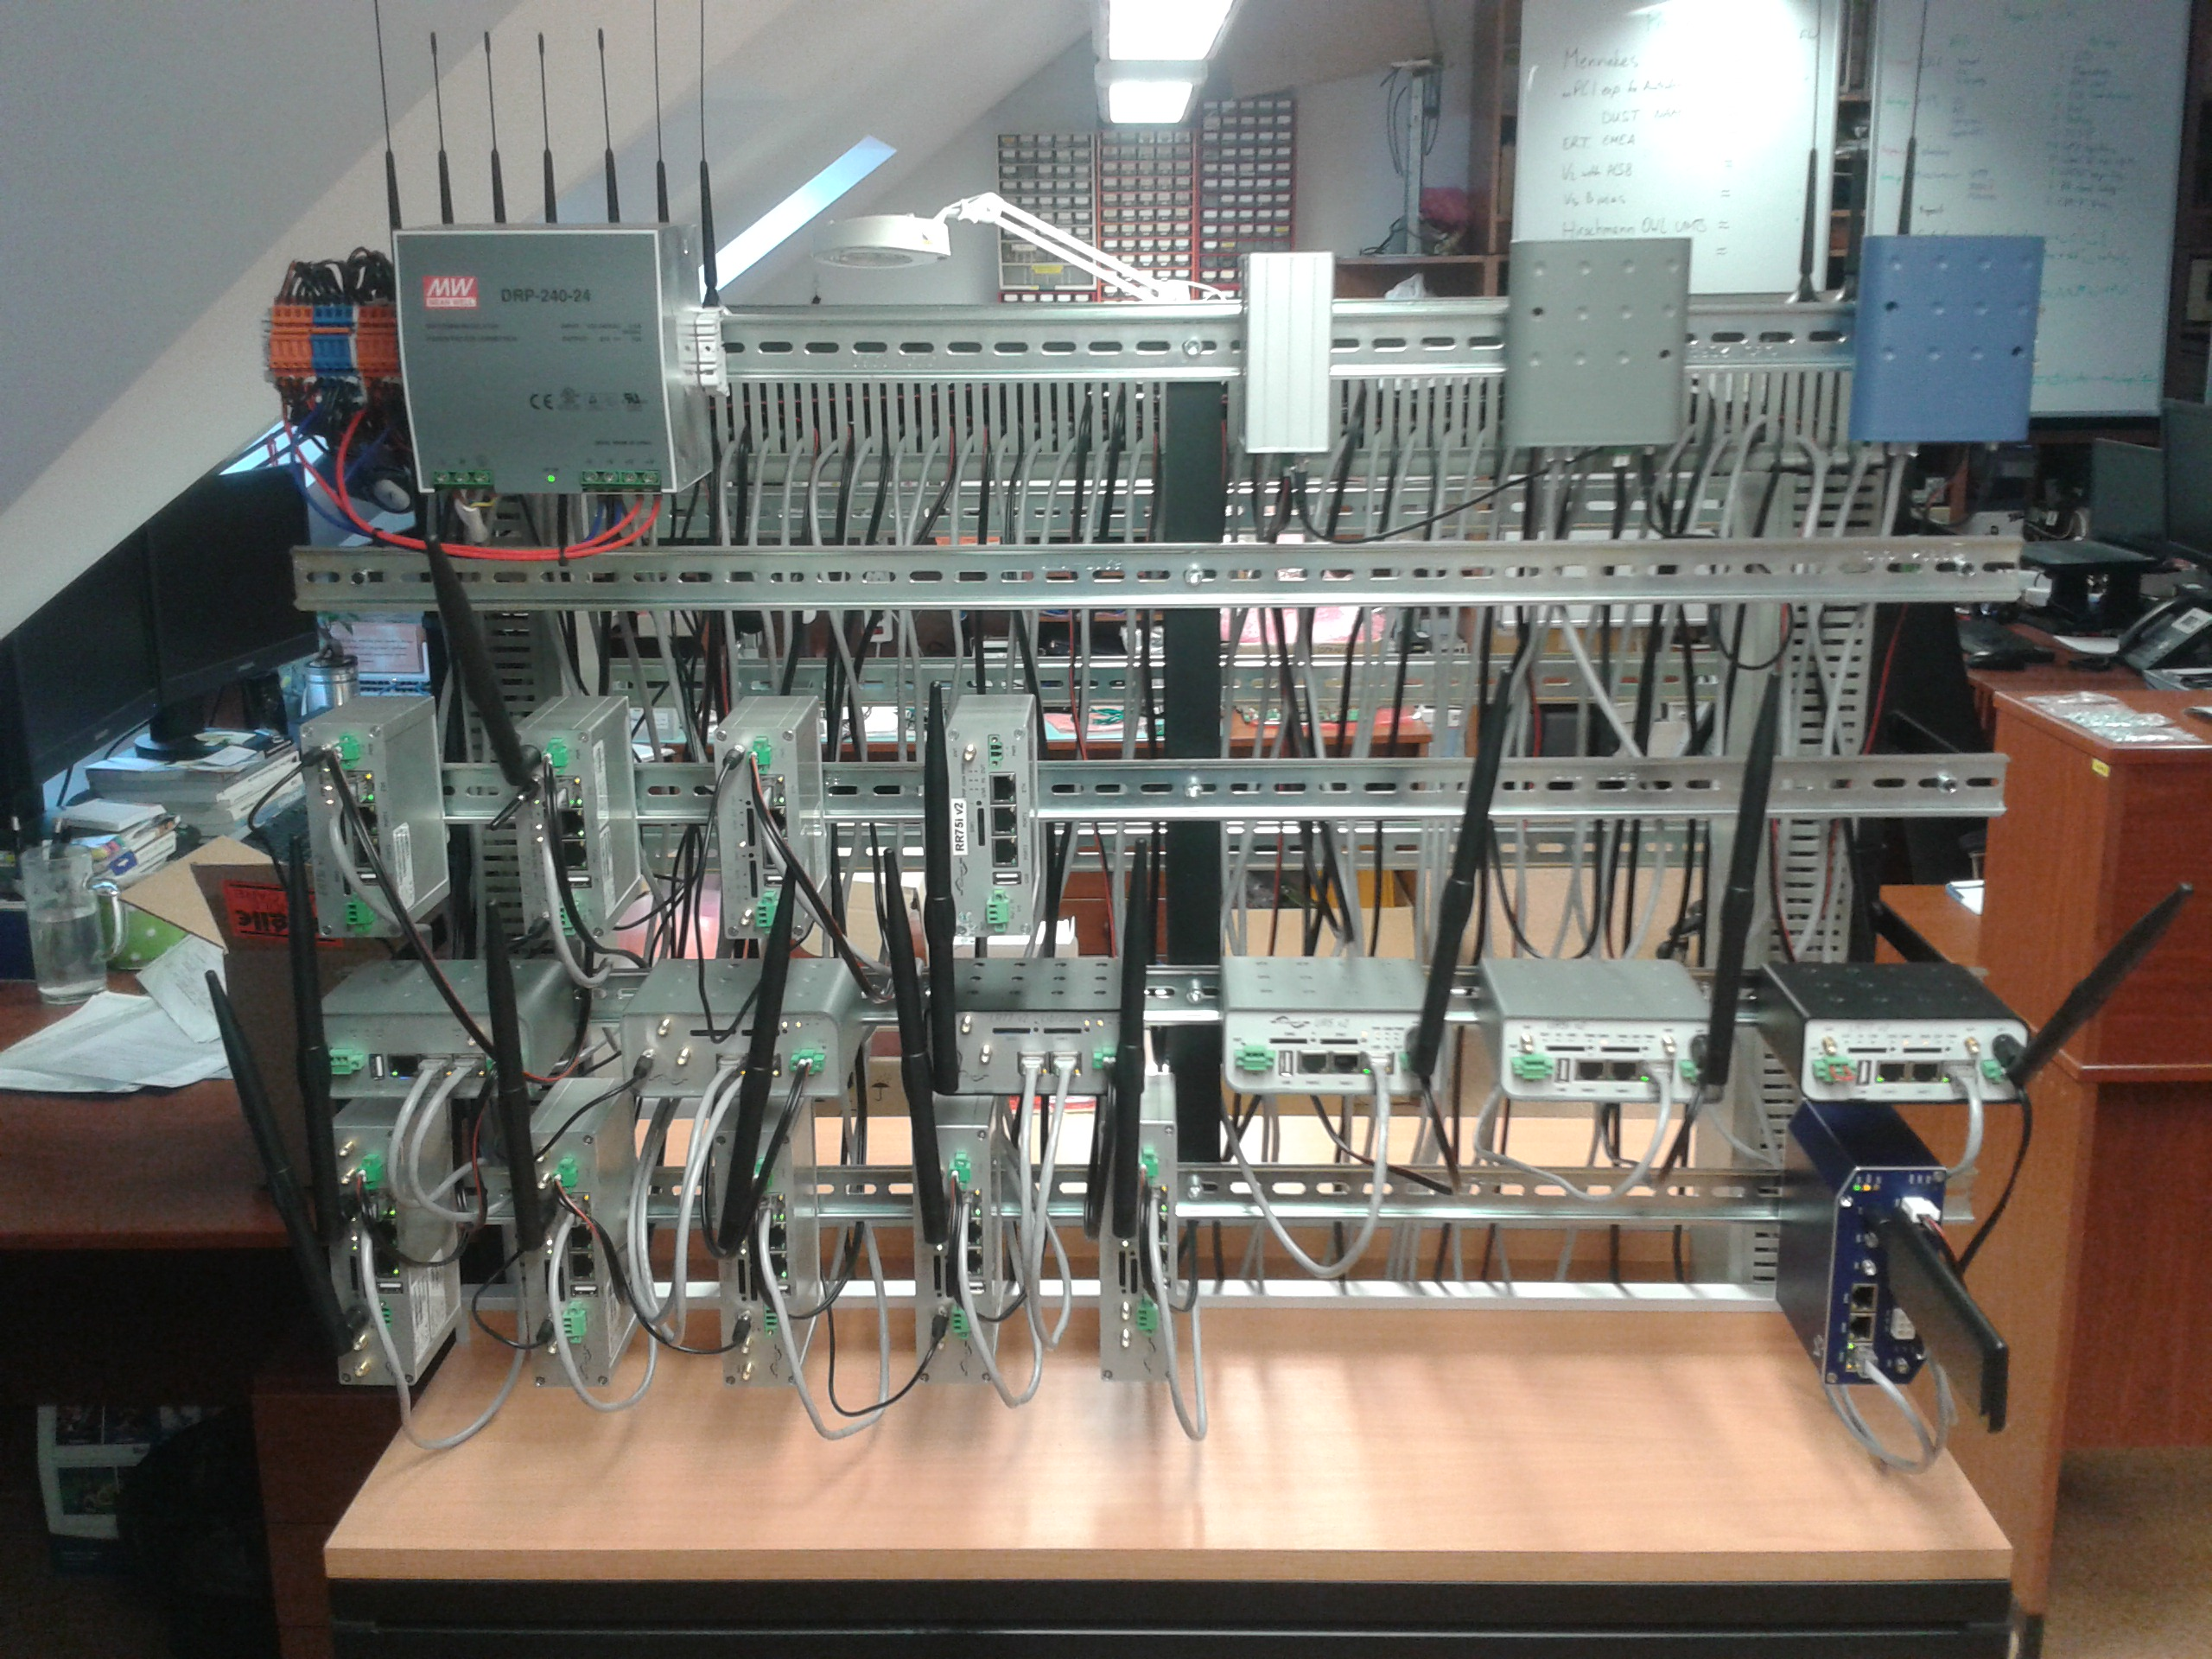
\includegraphics[width=\LW]{stojan4}
  \caption{Dokončené testovací pracoviště}
  \label{fig:stojan4}
\end{figure}

\begin{figure}[h]
  \centering
  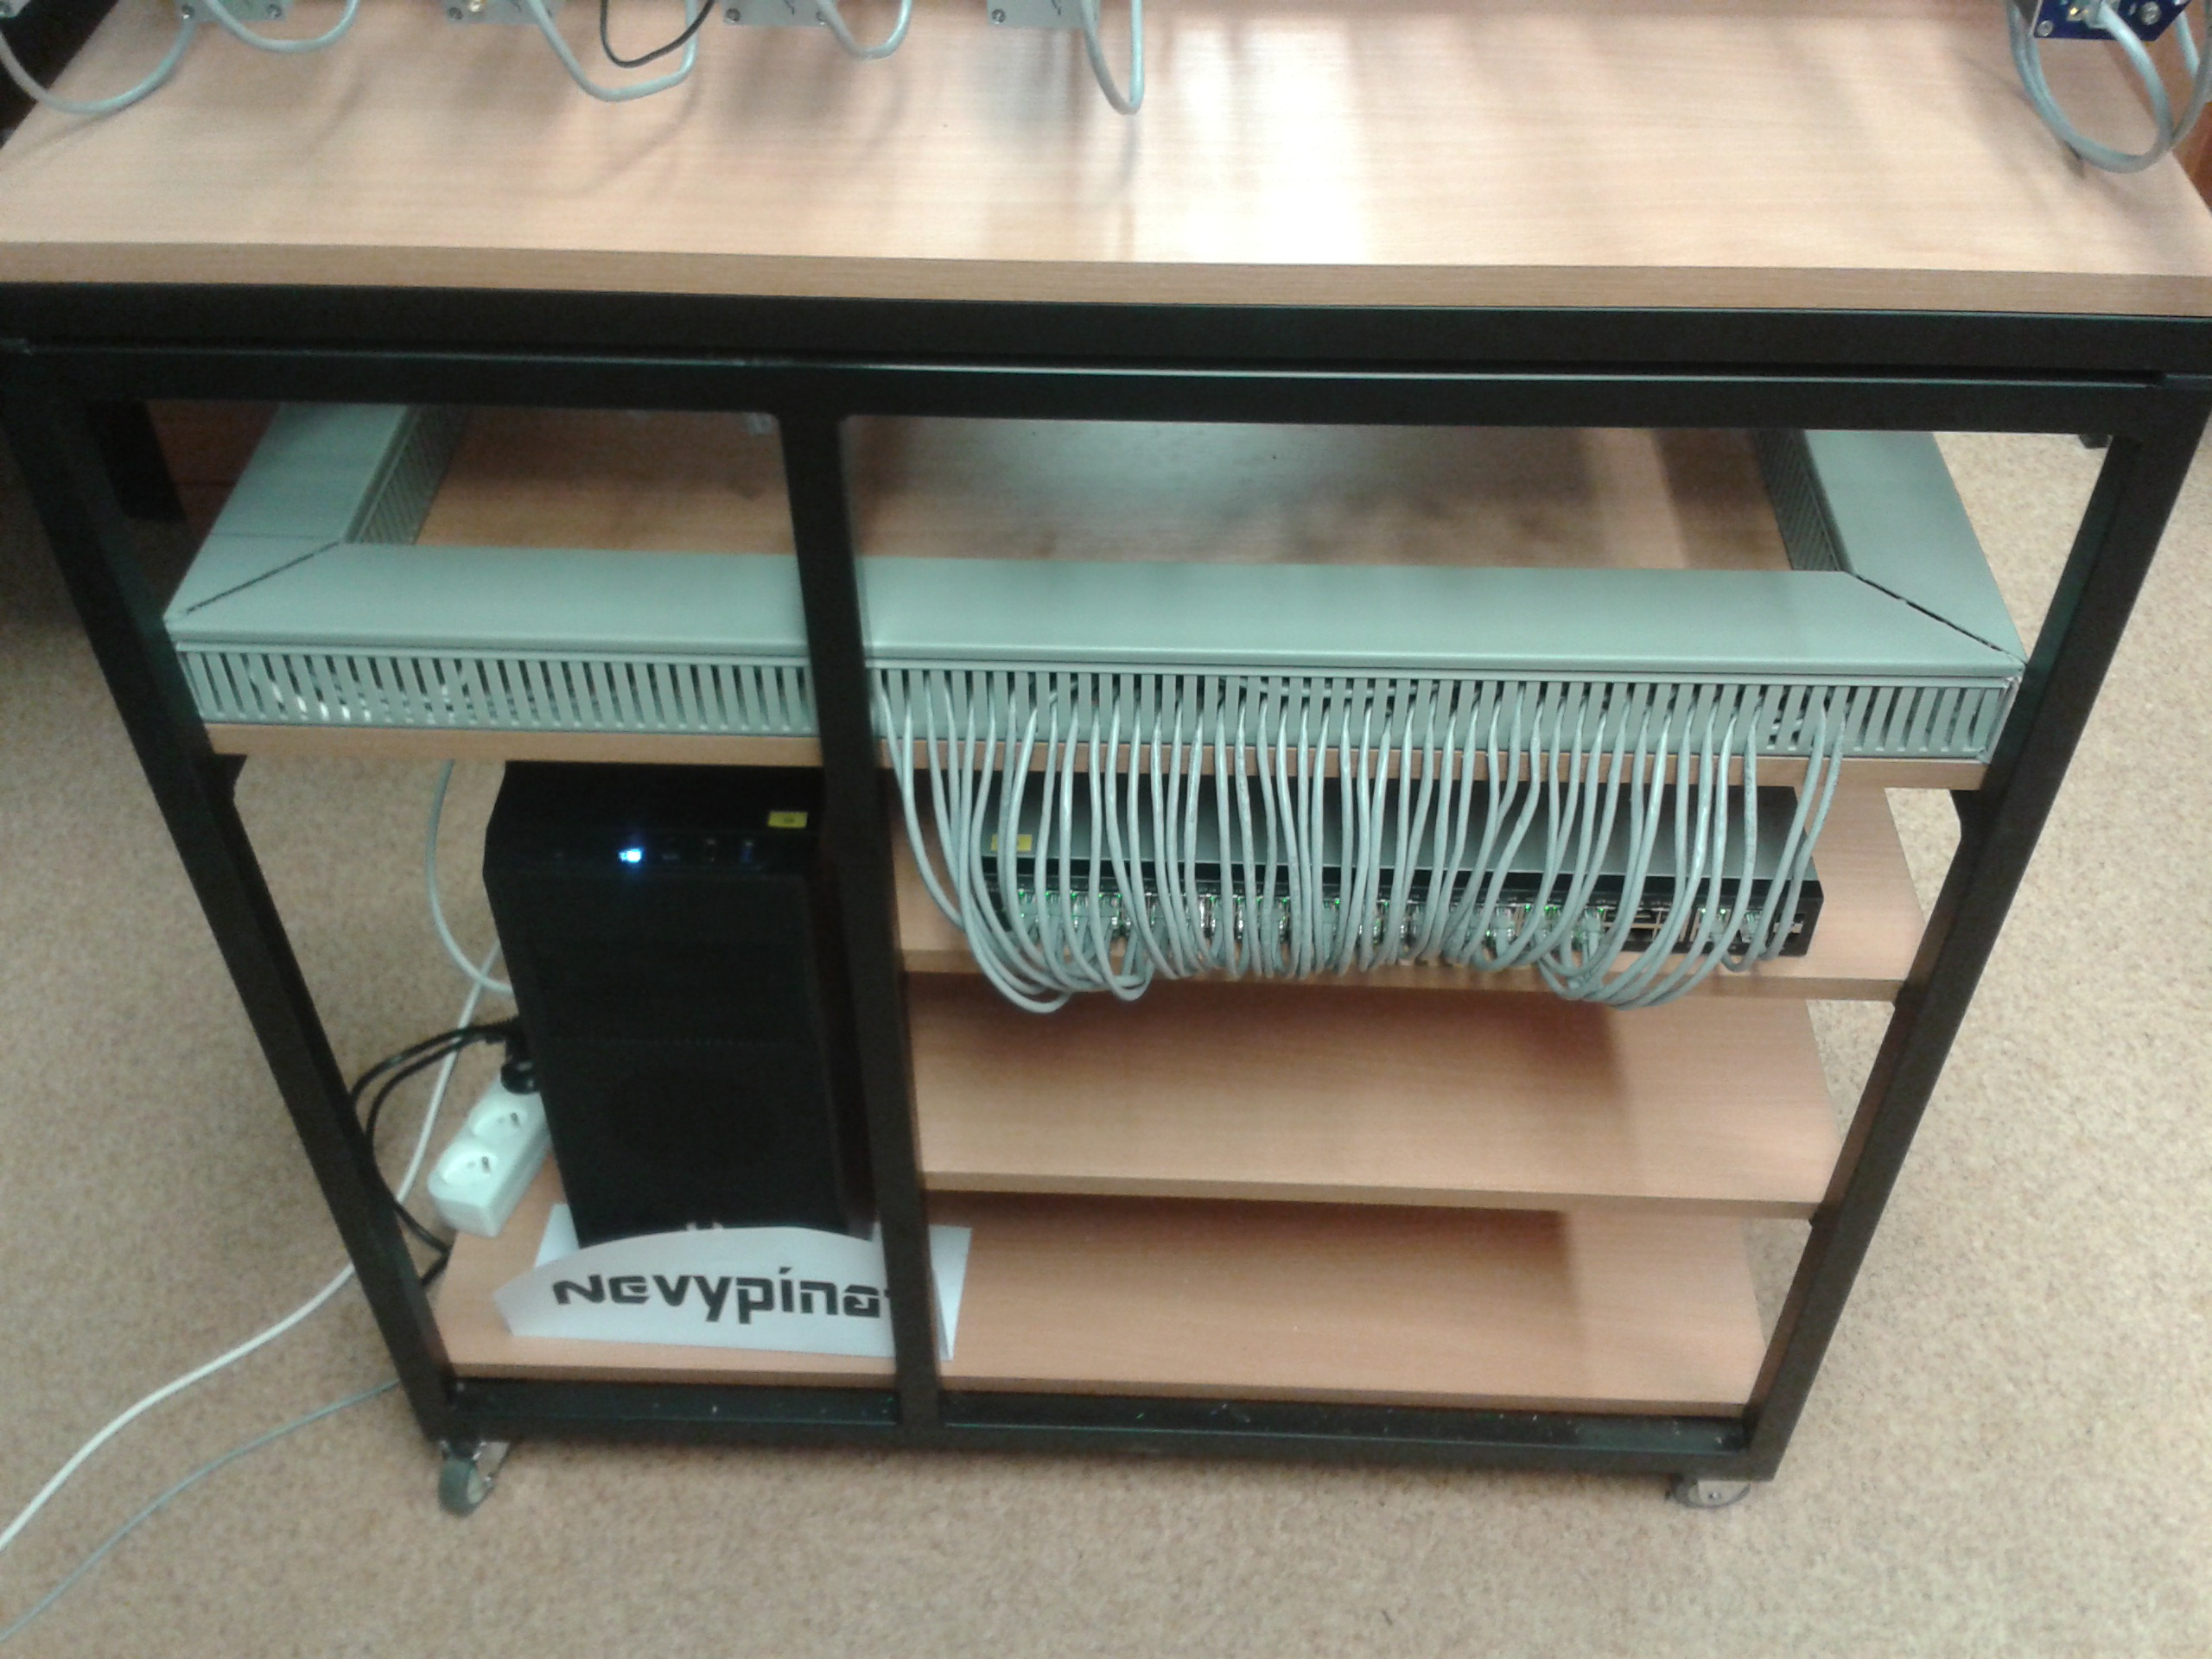
\includegraphics[width=\LW]{stojan3}
  \caption{Dokončené testovací pracoviště}
  \label{fig:stojan3}
\end{figure}



\endinput

  \chapter{Návrhy na budoucí rozšíření}
Testovací laboratoř je v nynějším stavu již plně funkční a pravidelně testuje základní funkcionality všech výrobků zde umístěných. Pomocí testovacího API lze snadno doplňovat nové testy testující další funkcionality. Psaní nových testovacích procedur jsem předvedl i testovacím pracovníkům a ti již zkouší psát nové testovací procedury. Nová zařízení lze jednoduše přidávat nastavením jejich základních vlastností a přiřazením podporovaných funkcionalit, čili vytvořením jejich modelů.

Pro zvětšení objemu testovaných funkcí a tím i zlepšení kvality samotného testování by bylo vhodné testovací systém dále rozvíjet ve směru psaní nových testů. Nové testy by měly testovat všechny jednotlivé funkce routerů. Při dopisování nových testů občas může vzniknout požadavek na nový program testovacího API, avšak tyto požadavky by měly postupem času vymizet. Největším zásahem do testovacího API, který bude muset být v budoucnu udělán je vytvoření sady programů pro automatickou konfiguraci switchů. Ve směru dopisování nových testů nebude vývoj testovací laboratoře nikdy ukončen, jelikož se testované výrobky neustále vyvíjejí, tudíž testovací procedury budou muset být neustále dopisovány.

Dalším budoucím rozšířením bude testování všech dostupných rozhraní routerů. Nyní jsou testovány pouze všechny Ethernet rozhraní. V dalších fázích bude přidáno testování všech sériových rozhraní zapojením zařízení do testovacích měřáků. Pro účely testování vstupů a výstupů bude potřeba vyvinout přípravek, kde na jedné straně bude komunikační rozhraní pro komunikaci s testovacím serverem a na druhé straně bude řada nastavitelných binárních vstupů a výstupů. Vstupy a výstupy tohoto přípravku budou propojeny se vstupy a výstupy všech testovaných zařízeních.

Správnou spolupráci hardwaru se softwarem je možné kontrolovat například měřením spotřeby každého zařízení po nahrání nového firmwaru. Tato hodnota může být také použita k určení průměrných spotřeb nových výrobků. Pro měření spotřeby bude do testovací laboratoře umístěn měřák s jakýmkoliv komunikačním rozhraním pro připojení do testovacího serveru, nejlépe s Ethernet rozhraním. Dále bude navrhnuta speciální deska, jejíž vstupem bude napájecí napětí pro všechny zařízení testovací laboratoře a komunikační rozhraní pro komunikaci s testovacím serverem. Výstupem desky budou napájecí napětí pro všechny testované zařízení. Měřící modul bude schopen postupně pomocí relé přivádět jednotlivá napájecí napětí přes ampérmetr a tím měřit spotřebu daného zařízení bez jejich vypnutí.

\endinput

  \chapter{Závěr}
Cílem této práce bylo navrhnout, implementovat a ověřit funkčnost metodiku pro automatizované testování s využitím postupů testování podle modelů. Nejdříve byly rozebrány všechny dostupné pohledy na testování. Ze všech metodik byly vybrány způsoby testování implementované v testovacím systémem. Implementována bylo integrační a systémové testování všech vyráběných výrobků, ostatní úrovně testování by nepřinášely takový přínos u konkrétních testovaných výrobků. Další použitá metodika testování výchází ze samotného zadání práce a je to testování podle modelů. Každému zařízení v testovací laboratoři je vytvořen model skládající se základních informací o daném zařízení a všech jeho podporovaných funkcí. Podle těchto informací se na všech zařízeních pouštějí a vyhodnocují testy.

V další fázi byly zkoumány dostupné nástroje pro všelijaké testování. Zde nebyl nalezen žádný nástroj který by byl schopen plně testovat zařízení pro které má být testovací systém postaven. I úpravy jakéhokoliv ze zkoumaných řešení by byli časově srovnatelné s vývojem nového vlastního systému pro systémové a integrační testování. Ve zbytku práce se tedy počítá s vývojem nového systému a použitím samostatných utilit v rámci modůlu nebo API testovacího systému.



\endinput

\stopBodyMatter

\startBackMatter
  \PrintBibliography
  %\PrintIndex % define index entry in the text by: \index{word}
\stopBackMatter

\end{document}

\endinput
